\documentclass[a4paper,11pt]{article}
%\usepackage[pdftex]{graphicx}
\usepackage{amsmath}
%\usepackage[latin1]{inputenc}
%\usepackage{hyperref}
%\usepackage[T1]{fontenc}
%\usepackage[utf8]{inputenc}
%%GD Quand je mets usepackage[utf8]{inputenc} je n'arrive plus à compiler la biblio
%J'ai essayé de débuger : je n'y suis pas arrivé
\usepackage{rotating}
\usepackage{setspace}
\usepackage{lscape}
\usepackage[round]{natbib}
\usepackage{multirow}
\usepackage{rotating}
\usepackage{vmargin}
\usepackage{epstopdf}
\usepackage{hyperref}
\usepackage{float}
\usepackage{caption}
\usepackage[tableposition=top]{caption}
\usepackage{ bbold }
\usepackage{ upgreek }
\usepackage{comment}
\includecomment{commentGD}
\usepackage[draft]{todonotes}
%%GDPour cacher les notes, \usepackage[disable]{todonotes}


%\usepackage[nolists, figuresfirst]{endfloat}
%\usepackage{sidefloat}

\setlength{\abovecaptionskip}{-8pt}

%\usepackage[usenames]{color}
%\definecolor{grey}{rgb}{0.35,0.35,0.35}
%\definecolor{webdarkblue}{rgb}{0,0,0.4}
%\definecolor{orange}{rgb}{0.7,0.2,0.05}


%\usepackage[pdfcreator={PDFLaTeX}, pdfproducer={PDFLaTeX}, pdfstartview=FitH, pdfpagemode=UseOutlines, pagebackref=false, colorlinks={true},
%citecolor={webdarkblue}, linkcolor={webdarkblue},
%urlcolor={webdarkblue}]{hyperref}



%\addtolength{\oddsidemargin}{-0.4in}
%\addtolength{\evensidemargin}{-0.4in}
%\addtolength{\textwidth}{0.8in} \addtolength{\topmargin}{-0.85in}
%\addtolength{\textheight}{1.7in}
\renewcommand{\baselinestretch}{1.2}





\setmarginsrb{3cm}{2cm}{3cm}{2cm}{0,5cm}{0,5cm}{0,3cm}{0,5cm}



% commands

\newcommand{\bi}{\begin{itemize}}
\newcommand{\ei}{\end{itemize}}
\newcommand{\be}{\begin{enumerate}}
\newcommand{\ee}{\end{enumerate}}
\newcommand{\bd}{\begin{description}}
\newcommand{\ed}{\end{description}}
\newcommand{\beqa}{\begin{eqnarray}}
\newcommand{\eeqa}{\end{eqnarray}}
\newcommand{\beq}{\begin{equation}}
\newcommand{\eeq}{\end{equation}}
\newcommand{\bs}{\bigskip}
\newcommand{\A}{$^a$}
\newcommand{\B}{$^b$}
\newcommand{\C}{$^c$}
\begin{document}



\title{\textsc{Beyond the Iceberg Hypothesis: \\Opening the Black Box of Transport Costs}} %\thanks{We are especially grateful to XXX. Part of this research was funded by the French Agence Nationale de la Recherche (ANR), under grant ANR-11-JSH1 002 01. Finally, any remaining errors are ours.}}}
%We also thank participants at the EEA 27\textsuperscript{th} Congress (Oslo), ETSG 13\textsuperscript{th} meetings (Copenhagen), INFER Workshop (Orleans), 45\textsuperscript{th} Congress of the Canadian Economic Association (Ottawa), IAW Workshop (Tubingen), and seminars at WTO, Strathclyde University, OFCE and EQUIPPE-University of Lille.
\author{Guillaume \textsc{Daudin}\thanks{%
Universit\'{e} Paris-Dauphine, PSL Research University, LEDa-DIAL, UMR 225, France \&
SciencesPo, Observatoire Français des Conjonctures \'{E}conomiques (OFCE), France}  \qquad J\'{e}r\^{o}me \textsc{H\'{e}ricourt} \thanks{Universit\'{e} de Lille - LEM-CNRS UMR 9221, France \& CEPII, France}\qquad Lise \textsc{Patureau}\thanks{Universit\'{e} Paris-Dauphine, PSL Research University, LEDa, France } }


\date{September 2016}
 \maketitle
\bigskip

\begin{abstract}
Following \cite{samuelson1954}, standard models of international trade have usually relied on modelling trade costs as an ad-valorem tax equivalent. However, many common empirical facts support the existence of additive costs. This paper provides a quantitative assessment of the size and the importance of the additive component in international transport costs.
Using SITC 3 and 4 digit cif-fab unit values over 1974-2013 taken from US imports data, we estimate the two components of transport costs by transport mode (air or ocean).
We find that additive costs are 2.85\% of fab unit values for ocean shipping (and ad-valorem ones 3.22\%). These values are respectively equal to 1.9\% and 2.5\% for air transport. Further, we show that taking additive costs into account improves the fit of the modelling of transport costs.
We also use the time dimension of our data to characterize the evolution of transport costs. After correcting for composition effects, we find that all types of transport costs have been roughly constant from 1974 to 1984 and then steadily decreased by 40\% over the period 1984-2013. Yet, this steady decline hides shifts in the relative importance of additive and ad-valorem. While most of the early decline in air transport costs can be explained by the ad-valorem component, this component nearly doubled in the 2000s. These results therefore confirm the importance of the additive component in accounting for international transport costs.
\end{abstract}

\thispagestyle{empty} \pagestyle{plain} \setcounter{page}{1}



{\normalsize JEL classification: F14, N70, R40\newline
Keywords: Transport costs estimates, transport costs determinants, non-linear econometrics, period 1974-2013, additive transport costs }

{\normalsize \vspace{0cm} }

{\normalsize \titlepage }

{\normalsize \newpage }

%\begin{spacing}{1.5}

\section{Introduction}


\noindent Trade costs are central in international economic analysis. In particular, they are considered a major obstacle to international economic integration and international trade flows. According to \citet{Jacks08}, trade cost declines explain around 55\% of the pre-World War I trade boom and 33\% of the post-World War II trade boom, while the abrupt rise in trade costs explains the inter-war trade collapse. After 1950, average trade costs fell by 16\%, notably through the reduction of policy trade costs promoted through the GATT (WTO starting in 1995) multilateral agreements.
Based on panel data, \citet{novy13} finds  that U.S. trade costs with major trading partners declined on average by about 40 percent between 1970 and 2000.
Yet, several papers (mostly based on empirical estimates of the gravity equation) have shown that trade costs still remain a major obstacle to trade (e.g. \citealp{Head_Mayer04} and \citealp{Disdier_Head08}). Using data over 1989-2000, \citet{anderson_wincoop_jel} thus estimate that average international trade costs for industrialized countries represent a 74\% markup over production costs.

Defined as the costs associated with the exchange of goods across national borders, trade costs are usually split into transaction costs (information costs, contract enforcement costs, costs associated with the use of different currencies...), policy costs (tariff  and non-tariff costs), time costs (time to ship goods) and transport costs \emph{per se}. In this vein, \citet{anderson_wincoop_jel} obtain that the 74\% markup made by international trade costs can be divided between 44\% for border-related trade barriers and 21\% for transportation costs. This last figure suggests that the share of transport costs in the consumer price of manufactured goods is substantial.
\citet{Behar_Venables} obtain that the elasticity of trade with respect to freight costs is sizeable, by around -3. If much of trade-policy barriers have been removed over the second half of the 20th century, these findings point out that the transport costs component of the overall trade costs remain large and deserve attention. This is accordingly the focus of the paper.\smallskip

\todo{reprendre slides presentation LEDa pour la motivation de la question.}

Following \citet{samuelson1954}, standard models of international trade have usually relied on modelling trade costs as an \emph{ad-valorem} tax equivalent (ie, as a constant percentage of the producer price per unit traded, part of the ``iceberg cost'' hypothesis\footnote{Rigourously speaking, the ``iceberg cost'' includes the ad-valorem costs and the fact that the costs are paid in terms of the good that is traded. As this last element is irrelevant in our case, we use the terme ``iceberg'' and ``ad-valorem'' interchangeably, as commonly made in the literature.}). However, many common empirical facts support the existence of additive costs. As documented by \citet{Irrazabal_2015}, pricing structure in shipping, additive tariffs, distribution costs... often exhibit (at least partly) an additive structure. The structure (additive vs ad-valorem) of transport costs is far from being anecdotal, as the literature has long emphasized its role in shaping the pattern of trade flows. The Alchian and Allen conjecture (\citealp{alchian}), that points out that the relative price of two varieties of some good will depend on the level of trade costs, does rely on the existence of additive costs: The relative demand for more expensive/higher quality product goods should increase with trade cost (``shipping the good apples out''). \citet{Lashkaripour-mimeo-2016} challenges this view. He finds supporting evidence for the \emph{ad-valorem} assumption by taking into account the fact that more expensive goods are systematically heavier and hence more costly to transport. One can yet be concerned by the generality of this result. By nature, his study is restricted to goods that are enumerated by items in the statistics (they represent 60\% of US imports). Furthermore, while the positive correlation between weight and price seems reasonable for goods from the second industrial revolution like cars, it is dubious in the case of ITC goods which importance has been rising since 1994 (the end point of Lashkaripour's study). Besides, a number of empirical papers provide a strong empirical support to the role of additive costs in international costs. Based on a firm-product-level database of French exporters, \citet{martin2012} finds that firms charge higher fas unit values on exports to more remote countries, in contradiction with the ad-valorem hypothesis. \citet{hummels_skiba} estimate the elasticity of freight rates with respect to price to be well below unity. Also, their estimates imply that doubling freight costs increases average fas export prices by 80-141 percent, consistent with high quality goods being sold in markets with high freight costs. These findings deliver strong empirical support in favor of the Alchian-Allen conjecture.
\smallskip


Beyond the positive aspect, several recent papers also point out the normative implications of additive trade costs. \citet{sorensen2014} extends \citet{melitz}'s seminal model of international trade by including additive trade costs, in addition to the ad-valorem component. A key analytical result is that the welfare gain from a reduction in trade barriers is higher for a decrease in additive costs than a decrease in ad-valorem costs.\footnote{\textbf{donner l'intuition. Deformation des prix relatifs, TBC}} Calibrating on Norwegian firm-level data for 2004, \citet{Irrazabal_2015} find that an additive import tariff reduces welfare and trade by more than an identically-sized ad-valorem tariff. While these results suggest that important welfare gains can be achieved by reducing additive trade costs, not much progress has been done in quantifying such gains. One potential reason is the lack of an empirical characterization of the additive component of trade costs.\footnote{The one exception being \citet{Irrazabal_2015}, upon which we come back later.} One objective of the paper is to fill this gap. \bigskip


Our paper provides an empirical decomposition of the structure of transport costs over time, by explicitly distinguishing between ad-valorem and additive parts. In this respect, the paper is related to the literature that challenges the dominant role of iceberg costs in international trade.\footnote{On top of the previously cited papers about additive costs, our paper also relates to \citet{Alessandria-et-al-AER-2010}, \citet{Hornok-et-al-RES-2015} or \citet{Hornok-et-al-JIE-2015}, which point out the role of per-shipment costs (among which, administrative costs) in generating some ``lumpiness'' in international trade transactions.}
We quantitatively assess the size and the importance of the additive component in international transport costs, that we measure as the difference between the import and the export prices, based on the US Imports flows over 1974-2013. Therefore, we focus only on a subset of trade costs. Besides, in terms of transport costs \textit{per se}, our measure based on the gap between export and import prices omits the other dimension of transport costs related to the time value of goods in transit. According to \citet{anderson_wincoop_jel}, the 21\% markup over production costs coming from transport costs includes both directly measured freight costs (10.7\%) and 9\% tax equivalent of ``indirect'' costs related to the time value of goods on their way to their export market (including holding cost for the goods in transit, inventory cost due to buffering the variability of delivery dates, preparation costs associated with shipment size...). However, the evidence summarized in \citet{anderson_wincoop_jel} points to a persisting importance of direct transport costs, especially compared to other trade barriers: they remain more important than, e.g., policy barriers (8\% tax equivalent), language barrier (7\%) or information cost (6\%). \citet{Hummels_1999} mentions a bunch of papers which all point that transport costs pose a barrier similar in size, or larger than tariffs. In the same vein, \citet{limao_venables} highlight the importance of infrastructures for trade costs in general, through their impact on transport costs. Furthermore, our data is based on a single and reliable customs origin, and allows for a wide time and geographical coverage, while limiting the measurement errors coming from strategies inferring trade costs. Therefore, we strongly believe they may deliver useful and reliable insights on the structure of international trade costs.

Closely related to our paper is the work by \citet{Irrazabal_2015}, which develops a structural framework for inferring additive trade costs from firm-level trade data. Based on Norwegian exports in 2004, they find that additive costs are about 14\% of the median consumer price. Our paper complements their findings in many respects. While they study trade costs in general, our database implies that we focus on international transport costs. Similarly to them, our various results emphasize the important role of the additive component of international transport costs. Further, our empirical analysis allows us to provide a quantitative measure of the levels of both the iceberg and the additive trade costs. Last, we exploit exhaustive information about the imports flows of the US, over a large time span from 1974 to 2013. In this respect, our results deliver a broader view of the magnitude of additive costs in international trade over time. By exploiting the time coverage of our database, our paper is also related to the international trade literature that studies the patterns of trade costs over time, such as \cite{hummels2007} and \cite{Behar_Venables}. We also share in common with these papers to investigate the time trends of transport costs by transport mode (i.e., air or sea). Many argue that transport costs have substantially decreased with technological advance in transportation, infrastructure development and new communication technologies (see\citealp{Lafourcade_Thisse}). \cite{Glaeser04} find that, over the twentieth century, the cost of moving goods have declined by over 90\% in real terms. However, \cite{hummels2007} shows that the bulk of price declines in transportation comes from air transport, where average cost per ton-kilometer shipped dropped by 92\% between 1955 and 2004. Concerning ocean shipping, which represents the major part of world trade, decline in trade prices are much less obvious, a conclusion in accordance with the studies reviewed by \cite{Behar_Venables}. Our paper contributes to this debate. In particular, we show the importance of taking into account the additive component in characterizing the time trends of international transport costs. Our findings can be summarized in three main points.

First, our theoretically agnostic approach provides a fairly simple framework for measuring both ad-valorem and additive parts of transportation costs. We thus obtain that the mean values over 1974-2013 of iceberg costs are equal to 2.5\% and 3.2\% of the export price in air and ocean transport respectively, whereas the additive component amounts to 1.8\% and 2.9\%. To our best knowledge, our paper is the first to provide such an extensive quantitative measure of both ad-valorem and additive costs in total transport costs.\footnote{Given their database and their methodology, \citet{Irrazabal_2015} can only identify the ratio of the additive to the ad-valorem cost ($\frac{t_{ik}}{\tau_{ik}}$ in our terminology), that they interpret by expressing it in terms of the median export price by country-product ($\bar{\widetilde{p}}_{ik}$). By contrast, our estimation strategy enables us to uncover both values of the ad-valorem and the additive costs $\tau_{ik}$ and $t_{ik}$ separately, in terms of the country-product export price $\widetilde{p}_{ik}$.}  This represents a valuable insight for calibrating related models.

Second, we provide an empirical assessment of what standard international trade models lose by skipping additive transport costs. Quantitatively, the omission of the additive term leads to overestimate the ad-valorem component by roughly a factor 2. On average over the whole period, biased estimate for ad-valorem is 5\% for air and 6\% for vessel, while unbiased estimate is respectively 2.5\% and 3.2\%. We also show that taking additive costs into account significantly improves the fit of the modelling of transport costs, through various measures of ``goodness-of-fit'', for both transport modes and years.

Third, we exploit the time dimension of our database to document the patterns of transport costs over time. As pointed out by \cite{hummels2007}, we confirm the importance of the composition effects by country of origin and by product in shaping the patterns of transportation costs over time. After excluding the composition effects, we find that all types of transport costs have been roughly constant from 1974 to 1984 and then steadily decreased by 40\% over the period 1984-2013. Further, our results point out an important bias in the time trends of transport costs when additive costs are omitted. While transport costs seem to exhibit a larger decrease in air than in sea transport between 1985 and 2005 when only iceberg costs are modeled, this difference vanishes when additive costs are taken into account. These results therefore confirm the importance of the additive component in accounting for international transport costs.\smallskip

The paper is built as follows. \ref{sec:data_method} presents our data and our  methodology. Sections \ref{sec:results_decomposition} and \ref{sec:results_trends} report our results. In Section \ref{sec:results_decomposition}, we characterize the role of the additive component of transport costs. After reporting the mean values over the period (by transport mode), we show how introducing additive transport costs improves the modelling of transport costs. Section \ref{sec:results_trends} characterizes the trends in each component of transport costs (by transport mode) over the period 1974-2013. Section \ref{sec:conclu} concludes.

\section{Data Sources and Empirical Methodology \label{sec:data_method}}

\subsection{A measure of Transportation Costs}

Our analysis of transportation costs consists in exploiting the difference between commodity-level export and import prices, as in \cite{hummels2007} (among others). The database we use to construct our measure of transport costs comes from US annual Imports of Merchandise provided by the Census bureau\footnote{More information available at: \url{http://www.census.gov/foreign-trade/reference/products/catalog/fl_imp.txt}}, spanning from 1974 to 2013. We first use customs values, quantities and freight costs to recover free-alongside (fas) and cost-insurance-fret (cif) prices, by goods, country of origin and transportation mode.\footnote{The related literature commonly refers to the fob price rather than the fas price. While both are closely related, we refer to the fas price as the price considered by the US Foreign Trade Statistics.} More precisely, the (unit) fas price is computed as the total ``customs value'' in the US trade statistics divided by the shipping weight; in other words, it is the price for one kg of the good net of transportation costs. The cif price is then computed as the sum of the customs value and freight charges, once again divided by the shipping weight. Our dependant variable is finally computed as the ratio of the cif price divided by the fas price. Higher than 1, the variable provides therefore with a measure of transport costs as a proportion of the good's price, an \emph{ad-valorem} equivalent. This is a quite standard and widespread strategy, as emphasized by \citet{anderson_wincoop_jel}.

It is worth acknowledging that using this dataset encounters some limitations. First, it restricts our analysis to the study of international transport costs, as our measure of the cif-fas price gap only covers freight, insurance and handling costs. It is thus silent about the others dimensions of international trade costs, unlike \citet{Irrazabal_2015}. Further, in terms of transport costs \textit{per se}, our measure based on the cif-fas price gap omits the other dimension of transport costs related to the time value of goods in transit. According to \citet{anderson_wincoop_jel}, the 21\% markup over production costs coming from transport costs includes both directly measured freight costs and 9\% tax equivalent of the time value of goods in transit. In this respect, it is true that using this dataset embraces a partial view of international transport barriers.

Yet, we believe that our analysis delivers valuable insights on this topic. Indeed, using this dataset has (at least) three main advantages. First, this dataset delivers a strong statistical reliability arising from a single, trustworthy, customs origin. Based on customs declarations, the US Imports database inventories all imports (both values and quantities) by country of origin to the United states at the HS 10-digit level, with a concordance code to the SITC 5-digit coding system. In addition, the database reports information regarding freight, insurance and handling expenditures by transportation mode (ocean (or ``vessel'') and air). The first will be crucial to compute transport costs (see below), the second will allow to enlighten substantial differences in the dynamics of transport costs across transportation mode. Second, using this dataset allows us to have the import price of the good, next to the export price. This is highly valuable, as we can estimate both the \textit{levels} of the iceberg costs and of the additive costs. This strongly differentiates us from \citet{Irrazabal_2015}, who can only estimate the ratio of additive costs as a share of the median total consumer price. Third, this dataset is available over a long time span. We are thus able to exploit information on a yearly basis from 1974 to 2013. \cite{hummels2007} preceded us in investigating the time dimension of this database. However, our paper differentiates from his work in two main respects. First, we extend the time coverage to the more recent period up to 2013, while \cite{hummels2007} stops in 2004. As we show in Section \ref{sec:results_trends}, covering the time period over the recent years delivers interesting insights regarding the trends in air shipping costs. Second, we study the time trends of transport costs by disentangling the additive from the iceberg components. This proves to be important in the characterization of transport costs changes over time, in particular in air transport.\smallskip

We use sectorial price data at the 3-digit level, even if the data of transportation costs is available at a more disaggregated level. As detailed below, the use of a nonlinear estimator triggers computational limitations that limit the level of possible detail, especially when covering a long period of time.\footnote{Yet, we ensure the robustness of these results by conducting the estimations at the 4-digit level for some selected years. The selected years for the 4-digit level estimations are: 1974, 1977, 1981, 1985, 1989, 1993, 1997, 2001, 2005, 2009, 2013. Comparing different levels of aggregation is useful to check differences and the presence of biases precisely due to aggregation. We thus obtain no substantial difference between the estimation results conducted at the 3 and 4-digit levels. Estimation results at the 4-digit classification level are reported in Appendix ??.} Depending on the considered year, this leaves us with around 200 sectors sectors, from approximately 200 countries of origin.


\subsection{Empirical specification}

\paragraph{The estimated equation} Our purpose is to provide estimates over time of the size of ad-valorem and additive costs among total transport costs. To do so, we start from the equation that expresses the price $p$ of a good $k$ paid by the importer (import, or cif) a function of the producer price $\widetilde{p}$ (export, or fas), given both per-kg ($t$) and ad-valorem ($\tau$) transport costs, according to:

\begin{equation}
p = \tau \widetilde{p}+ t \label{eq:base}
\end{equation}

\noindent As usual in the literature, the iceberg trade costs are denoted $\tau$ (with  $\tau \geq 1$, $\tau=1$ meaning no ad-valorem trade costs), while additive trade costs are labeled $t$ (with $t \geq 0$, $t=0$ implying no additive costs).  Let us denote $i$ the origin country, and $k$, the product. Transforming the above equation (\ref{eq:base}) as ratio, we thus get the following equation at the root of our estimation:\footnote{We skip the year and transport-mode dimensions in the notations for reading convenience.}

\begin{equation*}
\frac{p_{ik}}{\widetilde{p}_{ik}} -1 = \tau_{ik} -1 +\frac{t_{ik}}{ \widetilde{p}_{ikz}} \label{eq:base_estimee}
\end{equation*}

\paragraph{Estimation Strategy} We follow \citet{Irrazabal_2015} by considering that \textit{1)} both ad-valorem and additive costs are separable between the origin country ($i$) and the product ($k$) dimensions, and \textit{2)} this separability is in a multiplicative way for the former and an additive way for the latter.In other words, $\tau_{ik}$ and $t_{ik}$ from Equation (\ref{eq:base_estimee}) are written as:\footnote{Notice that, given the magnitude or order of transport costs, assuming an additive or a multiplicative form does not make a substantial difference since, for small values (as we obtain), we have $\tau_i\times \tau_k \simeq (\tau_i-1)\times (\tau_k -1)-1$ and $t_i+t_k\simeq (1+t_i)\times(1+t_k)-1$.}

\begin{eqnarray}
\tau_{ik} &=& \tau_{i} \times \tau_{k} \label{eq:ad-valorem}\\
t_{ik} &=& t_{i} + t_{k} \label{eq:add}
\end{eqnarray}

\noindent As a result, our underlying theoretical equation is specified as:

\begin{equation*}
\frac{p_{ik}}{\widetilde{p}_{ik}}-1 =\tau_{i} \times \tau_{k} -1 +\frac{t_{i} + t_{k}}{ \widetilde{p}_{ikz}} \label{eq:theory_equation}
\end{equation*}

The ratio $\frac{p_{ik}}{\widetilde{p}_{ik}}$ has a lower bound of one, since by construction, the cif price $p$ cannot be lower than the fas price ($p_{ik}>\widetilde{p}_{ik}$). Taking into account this constraint in the estimation suggests that the error term should be always positive and multiplicative, as in:

\begin{equation*}
\frac{p_{ik}}{\widetilde{p}_{ik}}-1 =\left(\tau_{i} \times \tau_{k} -1+\frac{t_{i} + t_{k}}{\widetilde{p}_{ik}} \right)\times \exp(\epsilon_{ik})
\end{equation*}
\noindent where $\epsilon_{ik}$ follows an normal law centered on 0. Considered in logs, the above equation becomes:

\begin{equation}
\ln\left(\frac{p_{ik}}{\widetilde{p}_{ik}}-1 \right)= \ln \left(\tau_{i} \times \tau_{k}+\frac{t_{i} + t_{k}}{\widetilde{p}_{ik}}-1 \right) + \epsilon_{ik} \label{eq:equation0}
\end{equation}

The non-linearity of Equation (\ref{eq:equation0}) implies that it cannot be estimated using standard linear estimators. All estimates are thus performed using non-linear least squares.\footnote{The basis of the method is to approximate the model by a linear one and to refine the parameters by successive iterations. The intuitive criterion for convergence is that the sum of squares does not decrease from one iteration to the next. See \cite{Woolridge-Book-2001} for more details.} Yet, the use of a nonlinear estimator triggers computational limitations that limit the level of possible detail, especially when covering a long period of time. Confronted to this arbitrage, we retain the 3-digit level as our benchmark classification, even though data series are available at the 5-digit classification level ($k$). This drives us to estimate a modified version of Equation (\ref{eq:equation0}), according to:
\begin{equation}
\ln\left(\frac{p_{ik}}{\widetilde{p}_{ik}}-1 \right)= \ln \left(\tau_{i} \times \tau_{s}+\frac{t_{i} + t_{s}}{\widetilde{p}_{ik}}-1 \right) + \epsilon_{ik} \label{eq:estimatedequation}
\end{equation}
where $\tau_{i}$, $\tau_{s}$, $t_{i}$ and $t_{s}$ are the parameters to be estimated, i.e., fixed effects specific to each origin country $i$ and sector $s$ (at the 3-digit classification level), and $\epsilon_{ik}$ the residual centered on 0. To eliminate the potential influence of outliers, we excluded 5 percent of the upper and lower tails of the distribution in the regression variables. These cut-offs are aimed at eliminating reporting or coding errors. We estimate this equation for each year over the period 1974-2013, for each of the transportation mode reported (air or vessel), on a sectoral-origin country basis ($i,s$). Depending on the year considered, this leaves us with around 800 fixed effects to estimate by transport mode (at the 3-digit level).   \smallskip

One key objective of the paper is to characterize the importance of additive costs relatively to ad-valorem costs. Put it differently, what traditional models of international trade lose by ignoring additive costs? A natural way to answer this question is to perform estimations of Equation (\ref{eq:estimatedequation}) constraining additive costs $t$ to be equal to zero, and compare the fitting properties and the explanatory power of the models. For each year and transport mode, we thus estimate the two models: \textit{(a)} when transport costs are modeled as iceberg costs (Equation (\ref{eq:model_nlI})), and \textit{(b)} when transport costs are modeled as decomposed in the two dimensions of additive and iceberg (Equation (\ref{eq:model_IetA})):

\begin{eqnarray}
\ln\left(\frac{p_{ik}}{\widetilde{p}_{ik}}-1 \right)&=& \ln \left(\tau_{i}\times\tau_{s}-1 \right) + \epsilon^{nlI}_{ik} \label{eq:model_nlI} \\
%\ln\left(\frac{p_{ik}}{\widetilde{p}_{ik}}-1 \right)&=& \ln \left(\frac{t_{i} + t_{s}}{\widetilde{p}_{ik}}\right) + \epsilon^{nlA}_{ik} \label{eq:model_nlA} \\
\ln\left(\frac{p_{ik}}{\widetilde{p}_{ik}}-1 \right)&=& \ln \left(\tau_{i} \times \tau_{s}-1 +\frac{t_{i} + t_{s}}{\widetilde{p}_{ik}}\right) + \epsilon_{ik} \label{eq:model_IetA}
\end{eqnarray}

After estimating Equation (\ref{eq:model_IetA}), we can re-built a measure of each component $\widehat{\tau}^{adv}_{is} = \widehat{\tau_{i}} \times \widehat{\tau_{s}}$ and $\widehat{t}^{add}_{is} = \widehat{t}_{i} + \widehat{t}_{s}$, that is country-product specific, by year and transport mode. Under Model (a), when assuming iceberg costs only (Equation (\ref{eq:model_nlI})), we proceed similarly to get $\widehat{\tau}^{nlI}_{is} = \widehat{\tau_{i}} \times \widehat{\tau_{s}}$.\footnote{In this case, notice that the equation could be estimated relying on a linear form. To preserve comparability of the results, we keep the same non-linear estimation method in both cases though.}$^{,}$\footnote{One may object that a comprehensive study of the structure of transport costs should also include the third model with only additive costs. This has driven us to estimate this case as well, in which case the estimated equation is written according to: $\ln\left(\frac{p_{ik}}{\widetilde{p}_{ik}}-1 \right)= \ln \left(\frac{t_{i} + t_{s}}{\widetilde{p}_{ik}}\right) + \epsilon^{nlA}_{ik}$. The main result that emerges is that the model with additive costs only is dominated (in terms of quality of fit properties) by the model with multiplicative costs only (which is itself dominated by the complete model (b), anticipating on further results. For sake of space saving, the results of this model are not reported in the paper. Of course, they are available upon request to the authors.} Similarly as \citet{Irrazabal_2015}, we take the average over the product-country dimension, using the values of each trade flow ($is$-specific) over total yearly trade as a weighting scheme. We thus recover a ``synthetic estimate'' of each type of transport cost: \textit{a)} $\widehat{\tau}^{nlI}$, \textit{b)} $\widehat{\tau}^{adv}$ and $\widehat{t}$, for each year and transportation mode. These results are reported in Section \ref{sec:results_decomposition}.

\todo{A un moment, parler du risque d'endogeneite entre tauik tik et ptildeik, dire que pas de pb. Dire ou?}


\section{Decomposing Transport Costs: The importance of the additive component \label{sec:results_decomposition}}

The objective of this section is twofold. First, we quantify the magnitude of transport costs over time (by transport mode), distinguishing whether the additive component $t_{ik}$ is included or not in the estimated equation (Equation (\ref{eq:model_IetA}) or (\ref{eq:model_nlI})). Second, we evaluate the importance of the additive component of in overall transport costs through the means of goodness-of-fit measures.


\subsection{Decomposing transport costs over 1974-2013}

Our first contribution to the literature is to provide estimates for the size of both the ad-valorem and the additive components of transport costs. Table \ref{tab:summary_results} reports a summary of our results. It displays the mean and median values of each type of trade costs (ad-valorem estimated alone, estimated along with additive costs and the additive component), as well as the associated standard deviation, averaged over the period 1974-2013, for estimation driven both at the 3- and 4-digit sectorial level.\footnote{In Appendix \ref{app:more_results}, we report similar results for a sample of years, for both transport mode, at the 3 and 4-digit classification level. Results for all years (available at the 3-digit level) are available upon request to the authors.}$^{,}$\footnote{We present the results for air at the 3-digit level removing the year 1989, as the estimation results reveal the presence of strong outliers that bias the estimates of transport costs upwards. Overall results (over the whole period) are not substantially affected if this year is included though. These results are available upon request to the authors.}

\begin{table}[htbp]
  \centering
  \footnotesize{
  \caption{Transport costs estimates: Summary \label{tab:summary_results}}
  \begin{center}
    \begin{tabular}{l|cc|cc}
      \hline \hline
    \multicolumn{5}{c}{Mean value over 1974-2013}   \\
    \# digit & \multicolumn{2}{c}{3 digits} & \multicolumn{2}{c}{4 digits ($^\ast$)} \\ \hline
    Mode  & Vessel & Air ($^{\ast \ast}$) & Vessel & Air \\ \hline
    \multicolumn{5}{l}{\textbf{With only Ad-Valorem Trade Costs} ($\widehat{\tau}^{ice}$, in \%)}  \\ \hline
    Mean  & 5.8 & 5.1 & 6.0 & 4.9 \\
    Median & 5.1 & 4.2 & 5.2 & 3.7 \\ \hline
    %Std   & 0.032 & 0.042 & 0.036 & 0.045 \\
    %Min. value & 1.003 & 1.001 & 1.003 & 1.000 \\
    %Max. value & 1.304 & 1.685 & 1.408 & 2.051 \\ \hline
    \multicolumn{5}{l}{\textbf{With Additive \& Ad-Valorem Trade Costs} } \\ \hline
   \textit{Ad-valorem term ($\widehat{\tau}^{adv}$, in \%)} & & & & \\ \hline
    Mean  & 3.2 & 2.5 & 3.3 & 2.4 \\
    Median & 2.8 & 1.8 & 2.8 & 1.6 \\ \hline
    %Std   & 0.023 & 0.023 & 0.025 & 0.026 \\
    %Min. value & 1.001 & 1.000 & 1.000 & 1.000 \\
    %Max. value & 1.227 & 1.474 & 1.264 & 1.537 \\ \hline
    \textit{Additive term ($\widehat{t}^{add}/\widetilde{p}$, in \%)}& & & &   \\ \hline
    Mean  & 2.9 & 1.8 & 2.8 & 1.9 \\
    Median & 1.9 & 0.7 & 1.7 & 0.8 \\ \hline
    %Std   & 0.041 & 0.034 & 0.039 & 0.034 \\
    %Min. value & 0.000 & 0.000 & 0.000 & 0.000 \\
    %Max. value & 2.941 & 13.303 & 3.197 & 11.440 \\ \hline
    \multicolumn{5}{l}{\textbf{Data} ($p/\widetilde{p}$, in \%) } \\ \hline
        Mean & 5.3 & 5.0& 5.6&3.9 \\
        Median & 4.3 & 2.0 & 4.4& 1.9 \\ \hline
        \# obs. & 29279 & 28207 & 29317 & 27680 \\
    \# origin country & 188 & 191 & 188 & 189 \\
    \# products & 230 & 211 & 666 & 567 \\  \hline \hline
  \end{tabular}
    \end{center}}
\parbox[l]{10cm}{\tiny{Notes: Statistics are obtained weighting each observation by its value relative to total trade flows. The additive term is expressed in fraction of fas price. ($^\ast$): Four 4-digit estimation: 0n selected years. ($^{\ast \ast}$): 1989 omitted in 3-digit estimation for air.}}
\end{table}%


Table \ref{tab:summary_results} yields the following comments. First, the magnitude of overall transport costs is sizeable. Over 1974-2013, they correspond to a mean increase of the export price by 5.8\% for ocean shipping, and by 5.1\% for air shipping. Air transport costs are smaller than sea transport costs. This is counter-intuitive, but certainly linked to selection effects.

% JH: XXX We have to discuss this: "Overall, these estimates are in line with the ones by \citet{Hummels_1999}, who finds on the same date that the all-commodities trade-weighted average transport cost is 3.8 percent of the fob price for the USA in 1994. More precisely, for this specific year, we find... something slightly higher...

%How do our results compare with other studies? Here, compare with Irrarazabal, Hummels and co.

Second, when decomposing transport costs into an additive and an ad-valorem component, we find that the per-kg cost dimension is sizeable. Over the whole period, additive costs are 2.9\% of the export price for ocean shipping  - and ad-valorem ones being equal to 3.2\%. These values are respectively equal to 1.8\% and 2.5\% for air transport. For both transport modes, the omission of the additive term seriously biases the ad-valorem term upward. In quantitative terms, the omission of the additive term leads to overestimate the ad-valorem component by roughly a factor 2.\todo{Ajouter un commentaire sur mean different de median, en comparaison avec les data.}

We extend further our analysis by using explicitly the time dimension of our analysis in order to assess the dynamics of our estimates over time. Figure \ref{fig:mult_alone_withadd} thus reports the mean value of the ad-valorem component, estimated alone (Dashed line, corresponding to Equation (\ref{eq:model_nlI})) and along with the mean value of the additive component (Plain line, corresponding to Equation (\ref{eq:model_IetA}), by transport mode.

\begin{figure}[htbp]
\caption{Ad-valorem Costs (Yearly mean value, 3 digits)}
\label{fig:mult_alone_withadd}
\begin{center}
\begin{tabular}{cc}
{\small (a) Air } & {\small (b) Vessel}\\
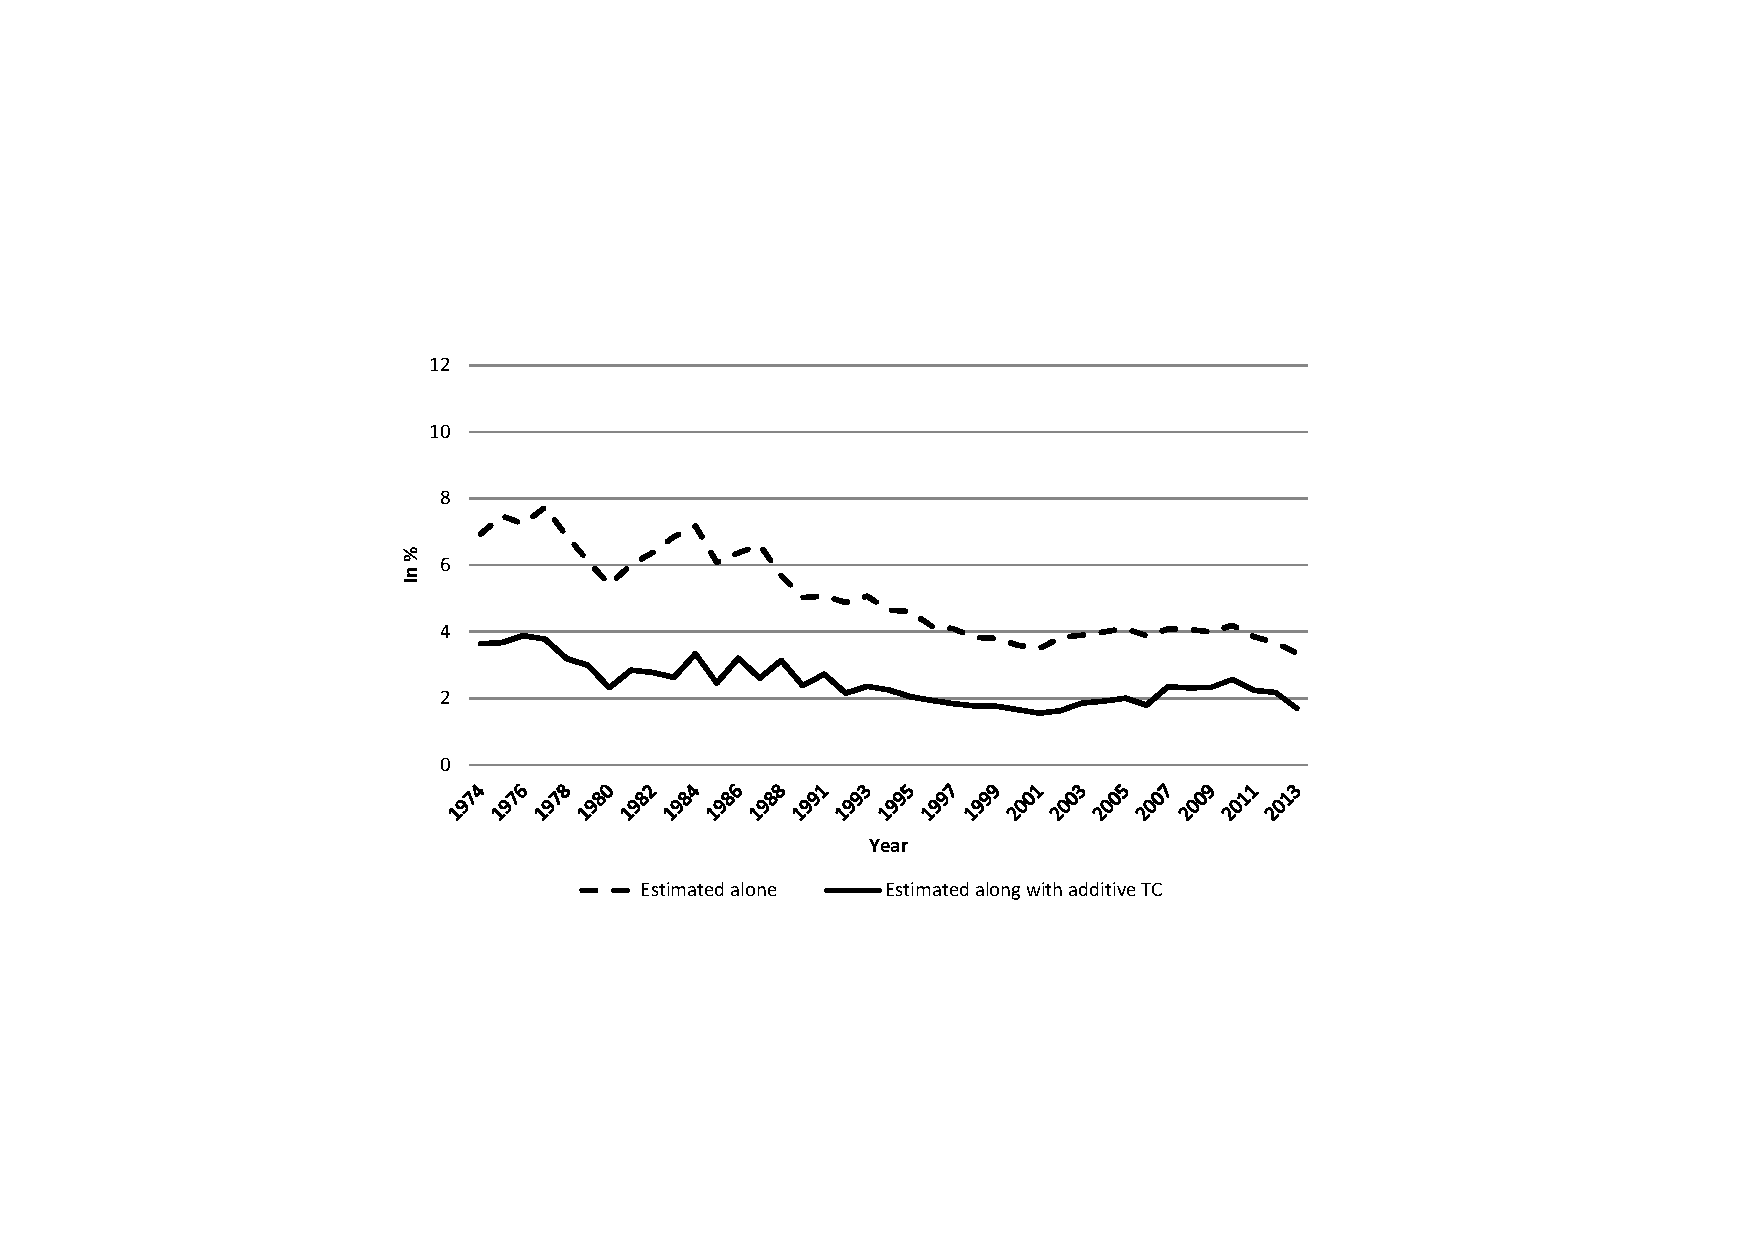
\includegraphics[width=3in, height=2.5in]{Fig1a_mult_air_3d.pdf}
& 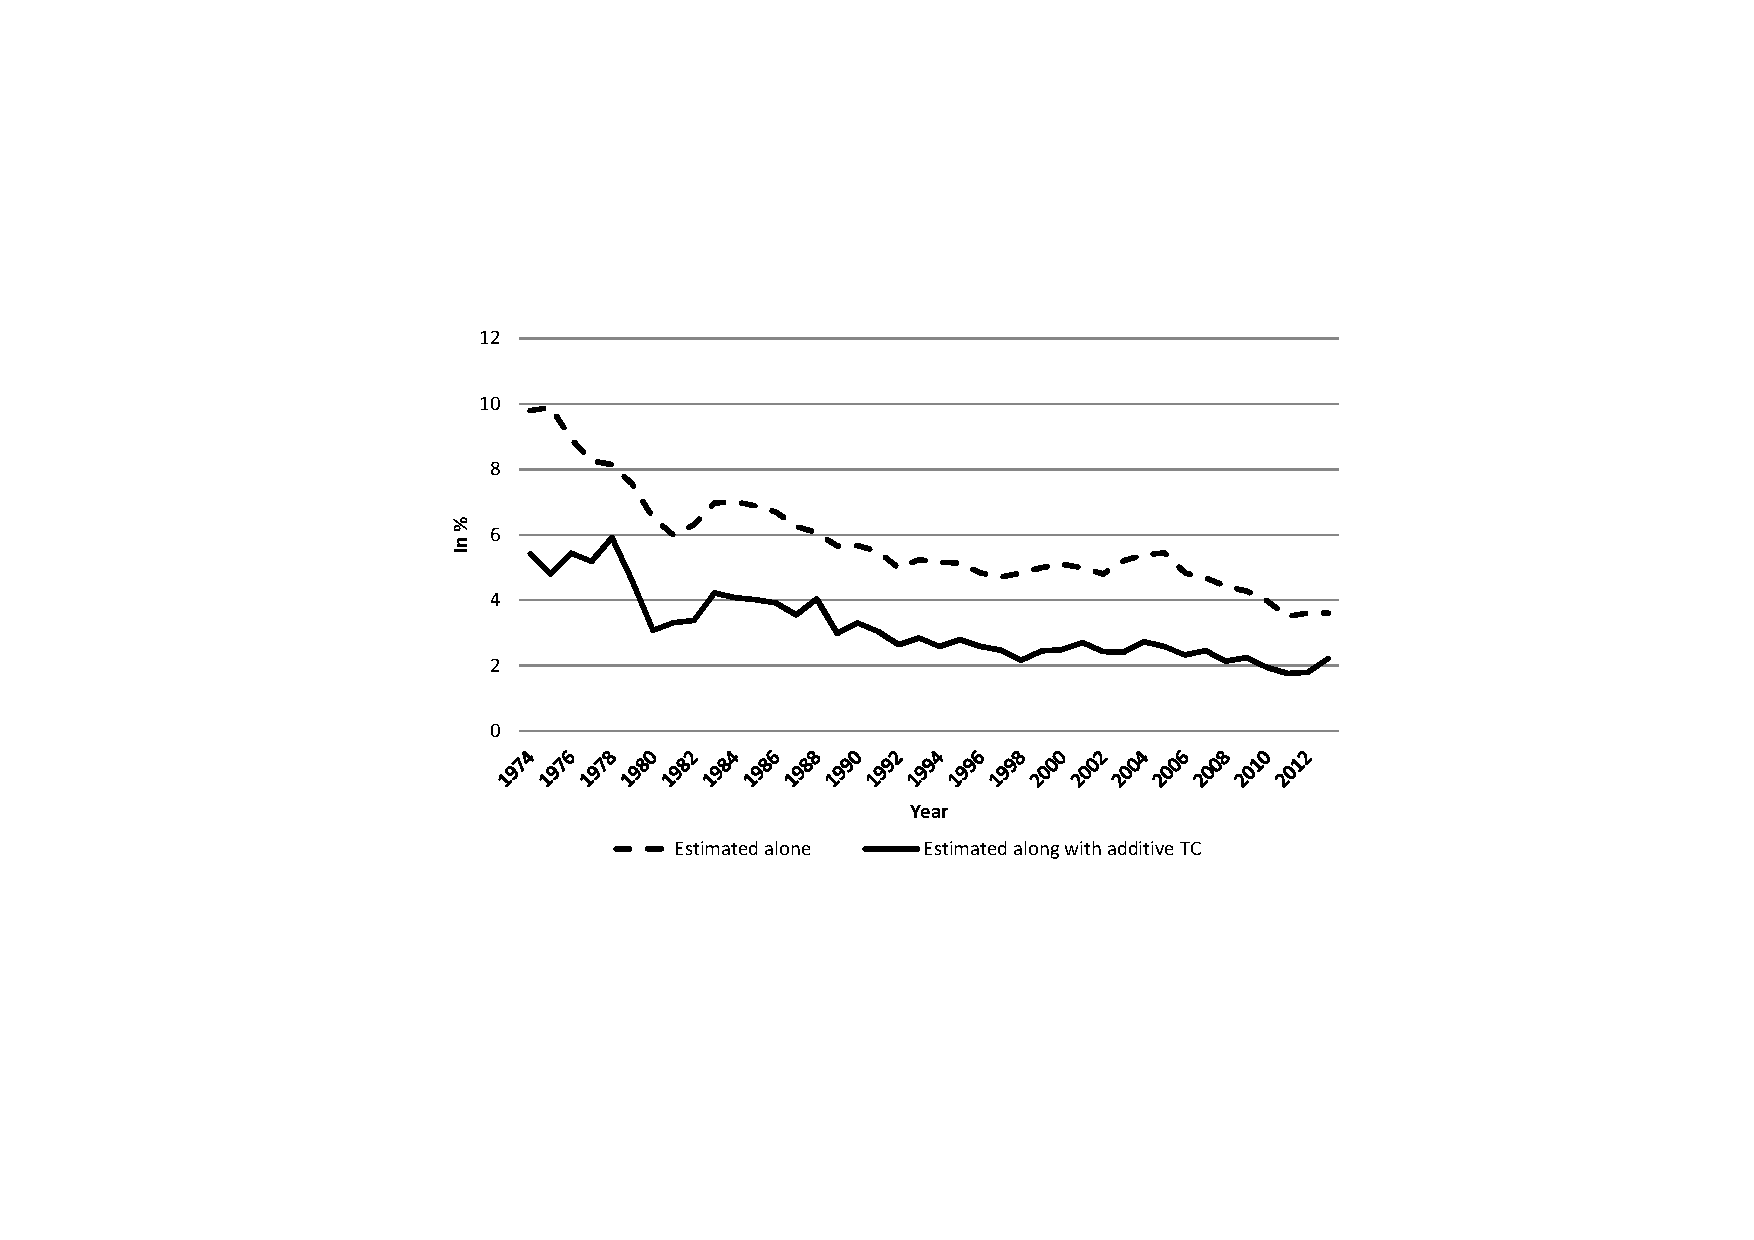
\includegraphics[width=3in,height=2.5in]{Fig1b_mult_vessel_3d.pdf} \\
\end{tabular}
\end{center}
\end{figure}

From Figure \ref{fig:mult_alone_withadd}, we can infer that the sizeable magnitude of additive costs also holds on a yearly basis. Further, Figure \ref{fig:mult_alone_withadd} reports that for Air, the size of the bias seems to decrease over time, while it appears rather stationary for ocean shipping. Put it differently, this suggests that the share of the additive component in total transport costs has decreased over time for air transport. To get a better picture on this, we study the shares of both ad-valorem and additive components in total costs, by transport mode and over time, based on Figure \ref{fig:decomp_TC_3d}.

\begin{figure}[htbp]
\caption{Decomposing Transport costs (Yearly mean value, 3 digits)}
\label{fig:decomp_TC_3d}
\begin{center}
\begin{tabular}{cc}
{\small (a) Air } & {\small (b) Vessel}\\
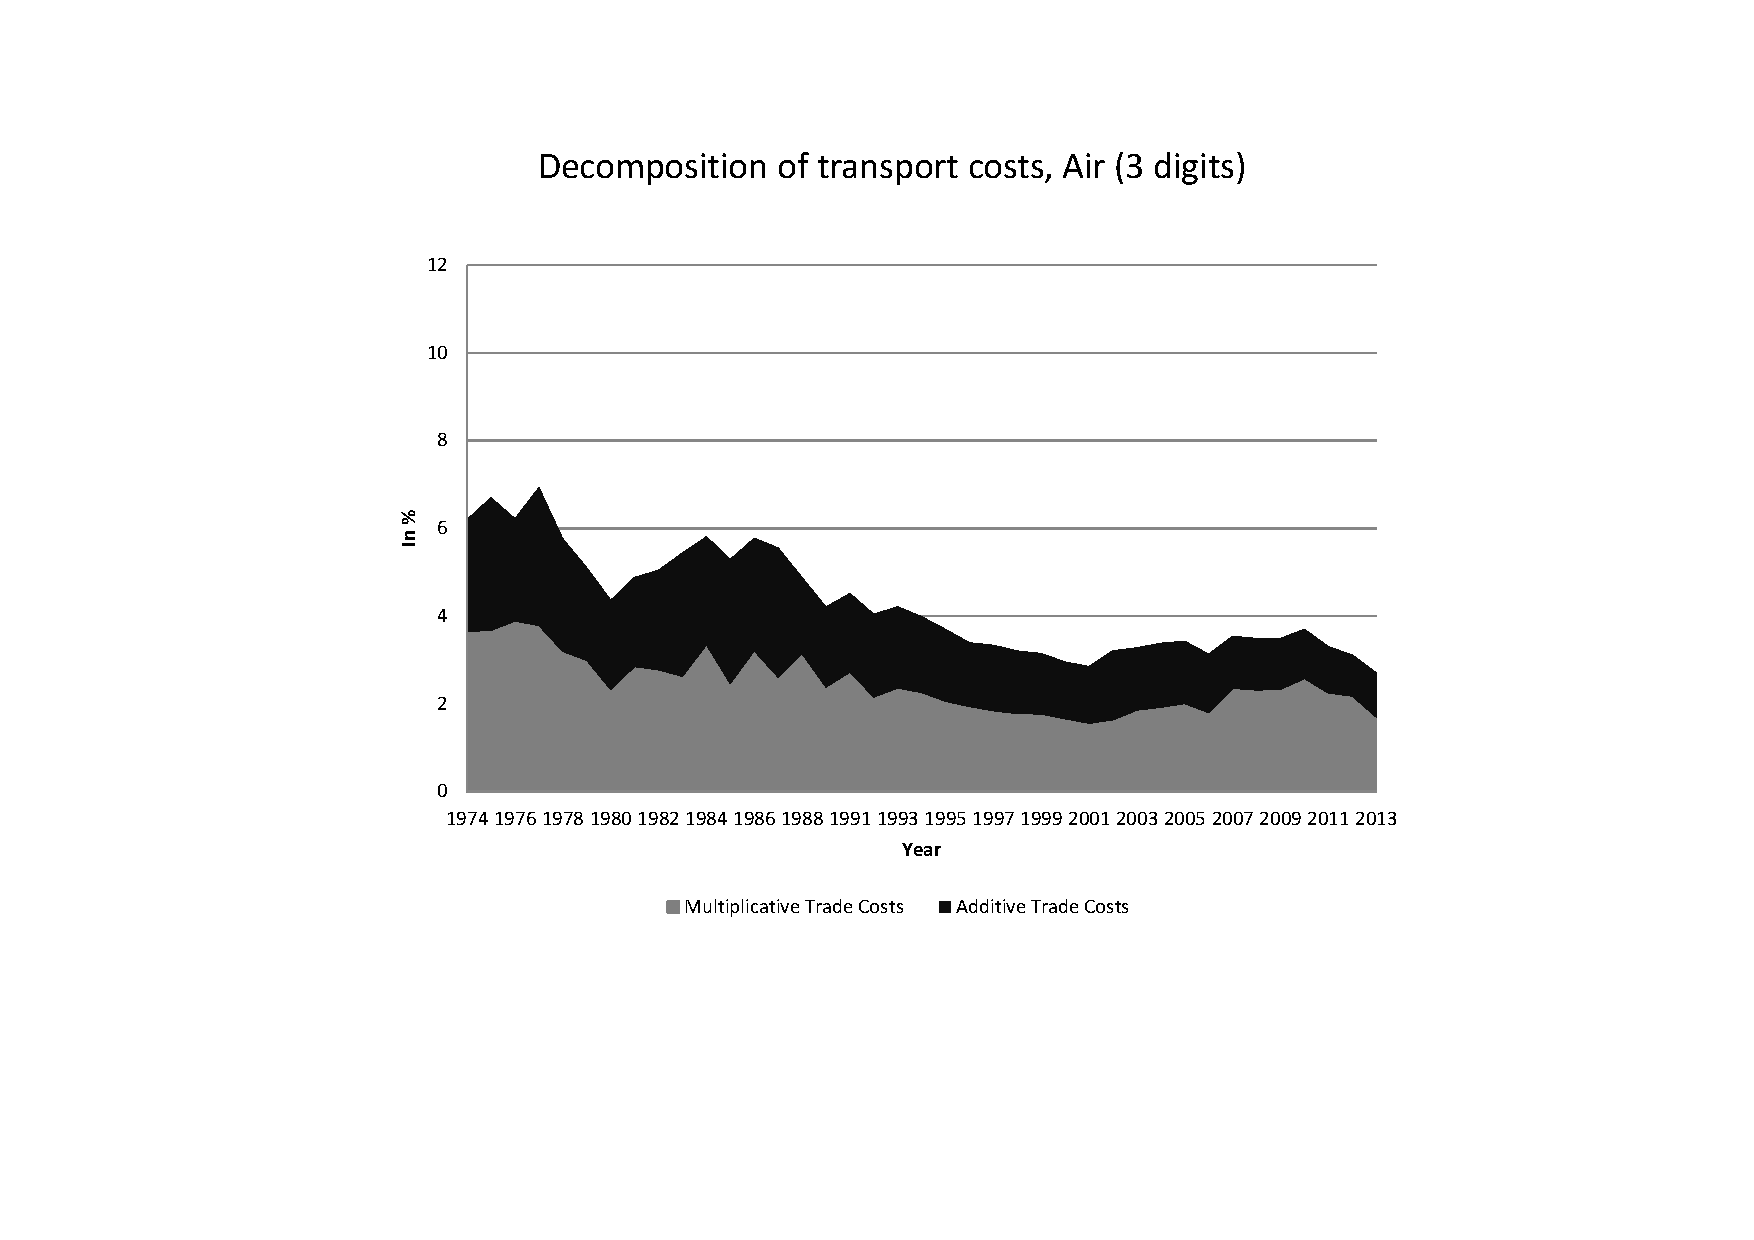
\includegraphics[width=3in, height=2.5in]{Fig2a_decompTC_air_3d.pdf}
& 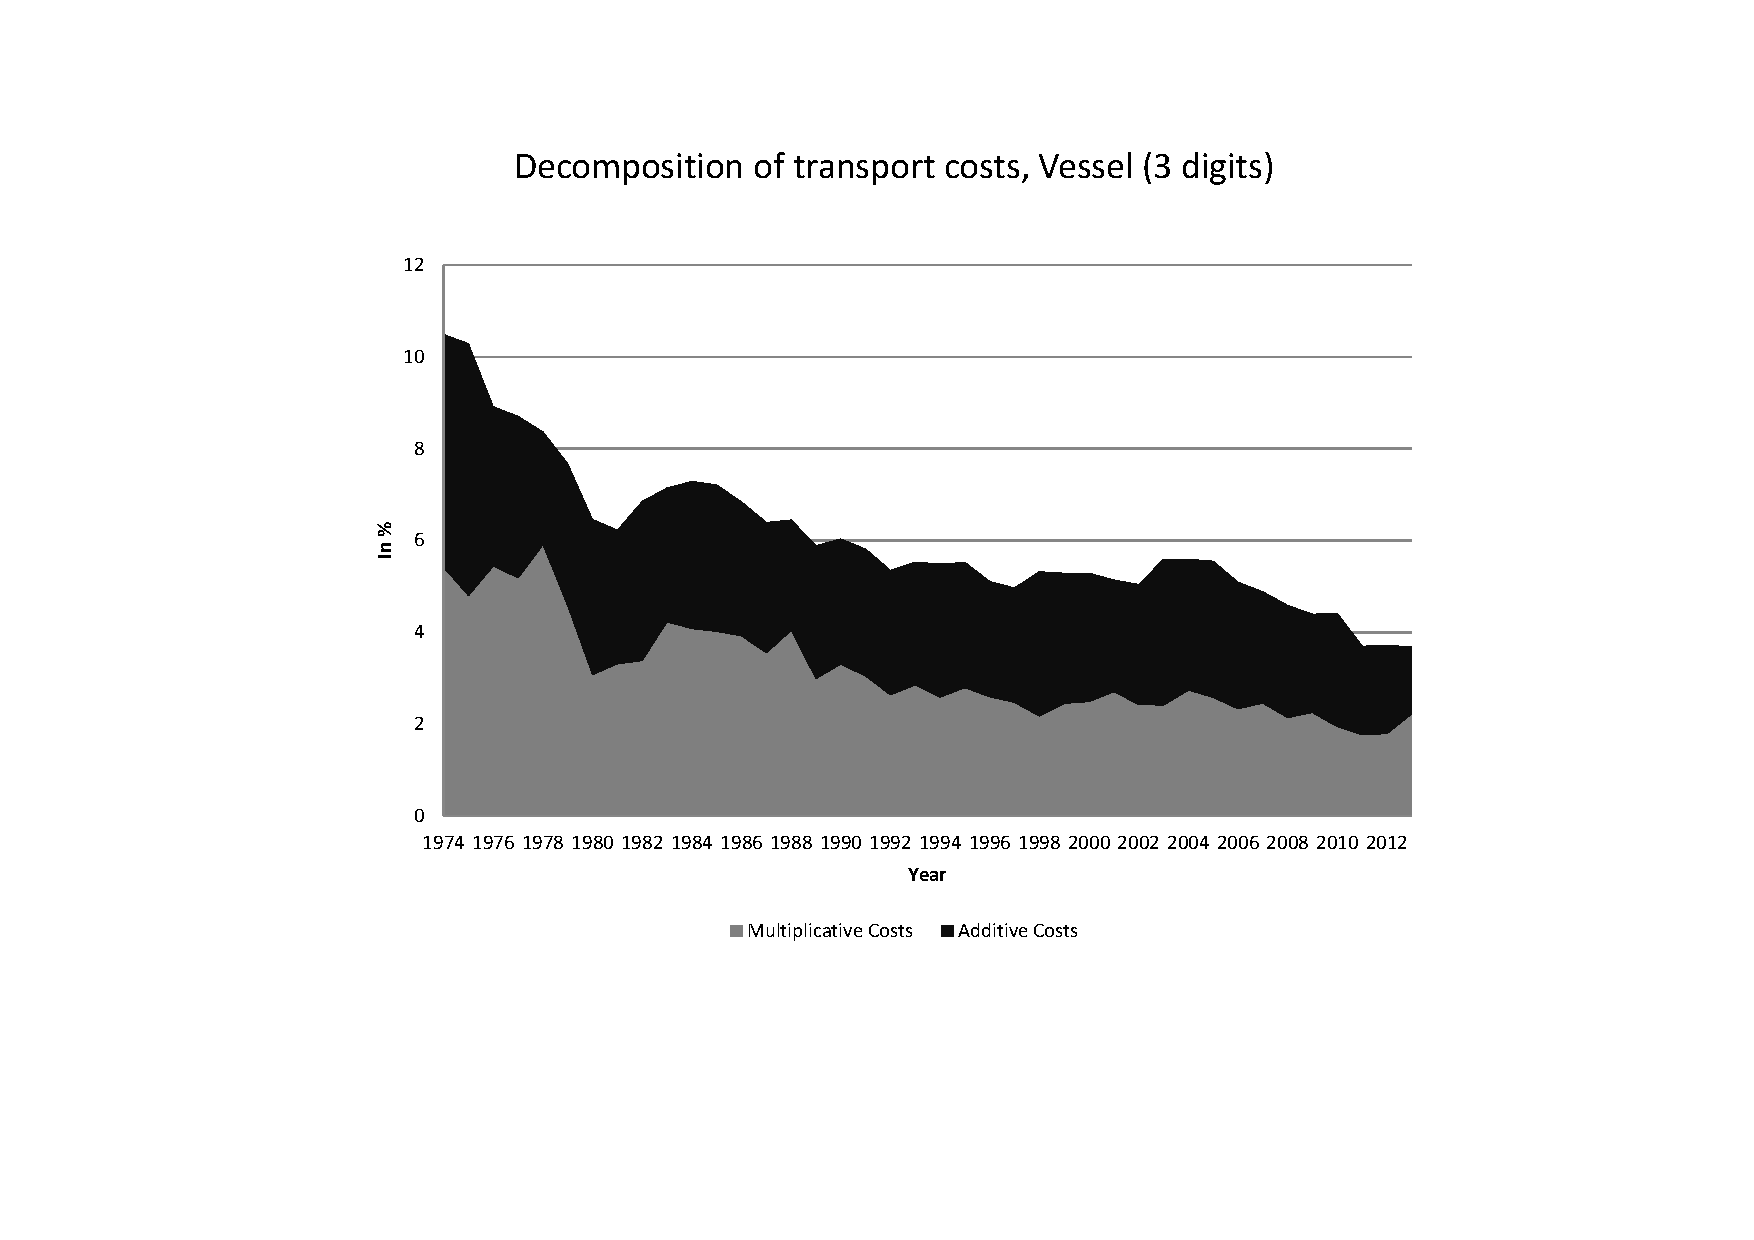
\includegraphics[width=3in,height=2.5in]{Fig2b_decompTC_vessel_3d.pdf} \\
\end{tabular}
\end{center}
\end{figure}

At this stage, two interesting comments can be made. First, the magnitude of transport costs is higher for ocean shipping than for air transport. This result holds considering ad-valorem costs alone (Figure \ref{fig:mult_alone_withadd}), as well as in presence of costs (Figure \ref{fig:decomp_TC_3d}), for all years throughout the period. Second, in both transport modes, the additive component appears of sizeable importance: As mean value over the period, it amounts to 48.2\% of total transport costs in Vessel, and 42.3\% in Air. We go on investigating this result further in the next subsection.\footnote{Figure \ref{fig:decomp_TC_3d} also delivers interesting results with respect to the time trends of transport costs. We come back to this aspect in Section \ref{sec:results_trends}.}\todo{Comparer avec la litterature. Cf AvW 2004 pure transport costs 11\% markup over production costs.}



\subsection{Assessing the importance of additive transport costs}

In this section, we explore the performances of each type of model (with and without additive costs) in fitting the observed cif-fas prices gap, in order to deliver a more systematic diagnosis about the importance of additive costs. To do so, we rely on several standard measures of fit. The first indicator is through comparing $R^{2}$. However, its use is far from being straightforward when evaluating non-linear estimates.\footnote{$R^2$ is based on the underlying assumption that the adjusted model is a linear one. In a non-linear context, $R^2$ is  strictly speaking inappropriate. However, if the error distribution is approximately normal, a standard metric like $R^2$ remains informative on the quality of adjustment.} This drives us to complement the goodness of fit diagnosis with three alternative measures. We provide the Standard Error of Regression (SER), which represents the average distance that the observed values fall from the regression line. Smaller values are better because it indicates that the observations are closer to the fitted line. We also report the log-likelihood function, and two measures derived, the Akaike Information Criterion (AIC) and the log-likelihood (LL) ratio test. A decrease in the log-likelihood function points to a better quality-of-fit. However, the likelihood function systematically decreases with the number of parameters included; the AIC criterion allows for correcting this overfitting by including a penalty in the computation of the statistic.\footnote{Precisely, the AIC stat is equal to $2 \times \textrm{number of parameters} - 2 \times \textrm{Likelihood} $.} The preferred model is the one with the minimum AIC value. Finally, the log-likelihood ratio test statistic compares systematically the likelihood of the Unrestricted model (\emph{UR}, including an additive term, i.e. Equation (\ref{eq:model_IetA}) and the Restricted one (\emph{R}, i.e. Equation (\ref{eq:model_nlI})). The null tested is that the two models are statistically equivalent. Results are reported in Tables \ref{tab:good_fit_air} and \ref{tab:good_fit_vessel}, for Air and Vessel respectively, at the 3-digit level.\footnote{Due to our time coverage, we do not report the results for all years (at the 3-digit level). The results for all years are available upon request to the authors.}\medskip



\begin{table}[htbp]
  \centering
  \caption{Air: Measures of Goodness-of-fit (3 digits)}
  \footnotesize{
\begin{center}
    \begin{tabular}{l|cccccc|c}
    \hline \hline
    Year  & 1974  & 1980  & 1990  & 2000  & \multicolumn{1}{c}{2010} & \multicolumn{1}{c}{2013} & Mean stat \\ \hline
    \multicolumn{8}{l}{\bf{$R^2$} }\\ \hline
    Term I only & 0.30  & 0.27  & 0.25  & 0.32  & \multicolumn{1}{c}{0.42} & \multicolumn{1}{c}{0.34} & 0.31 \\
    Terms A \& I & 0.59  & 0.65  & 0.63  & 0.64  & \multicolumn{1}{c}{0.51} & \multicolumn{1}{c}{0.46} & 0.60 \\ \hline
    \multicolumn{8}{l}{\textbf{SER}  }  \\ \hline
    Term I only & 0.79  & 0.86  & 0.81  & 0.84  & \multicolumn{1}{c}{0.86} & \multicolumn{1}{c}{0.92} & 0.85 \\
    Terms A \& I & 0.67  & 0.71  & 0.67  & 0.70  & \multicolumn{1}{c}{0.79} & \multicolumn{1}{c}{0.85} & 0.73 \\ \hline
   \multicolumn{8}{l}{\textbf{AIC criteria}}  \\ \hline
    Term I only & 35674.98 & 41170.98 & 60715.58 & 87492.55 & \multicolumn{1}{c}{102297.66} & \multicolumn{1}{c}{88191.87} & 70498.1 \\
    Terms A \& I & 31387.29 & 35738.39 & 52098.91 & 74954.88 & \multicolumn{1}{c}{95887.05} & \multicolumn{1}{c}{80873.72} & 62285.0 \\ \hline
    \multicolumn{8}{l}{\textbf{Log-likelihood}} \\ \hline
    Term I only & -17530.5 & -20253.5 & -29977.8 & -43341.3 & \multicolumn{1}{c}{-50746.8} & \multicolumn{1}{c}{-43692.9} & -34888.6 \\
    Terms A \& I & -15125.6 & -17263.2 & -25393.5 & -36788.4 & \multicolumn{1}{c}{-47277.5} & \multicolumn{1}{c}{-39751.9} & -30508.3 \\
    LL ratio & 4809.7 & 5980.6 & 9168.7 & 13105.7 & \multicolumn{1}{c}{6938.6} & \multicolumn{1}{c}{7882.1} & 8760.69 \\
    nb of restrictions & 355   & 369   & 393   & 426   & \multicolumn{1}{c}{426} & \multicolumn{1}{c}{427} & 402 \\
    p-value & 0.00 & 0.00 & 0.00 & 0.00 & \multicolumn{1}{c}{0.00} & \multicolumn{1}{c}{0.00} & 0.00 \\
    \hline \hline
 \end{tabular}%
    \end{center}}
  \label{tab:good_fit_air}%
 \parbox[l]{12cm}{\tiny{Notes: SER = Standard Error of regression; AIC = Akaike Information Criterion. $R^{2}$ between the log of predicted ratio and the log of the observed ratio. For the LL ratio test, the number of restrictions is equal to the number of parameters estimated, i.e., the number of partner countries plus the number of products. The mean statistics calculated as the average value over all years. }}
\end{table}%

\begin{table}[htbp]
  \centering
  \caption{Vessel: Measures of Goodness-of-fit (3 digits)}
    \footnotesize{
\begin{center}
\begin{tabular}{l|cccccc|c}
\hline \hline
Year  & \multicolumn{1}{c}{1974} & \multicolumn{1}{c}{1980} & \multicolumn{1}{c}{1990} & \multicolumn{1}{c}{2000} & 2010  & \multicolumn{1}{c}{2013} & Mean stat \\ \hline
\multicolumn{8}{l}{\bf{$R^2$} }\\ \hline
Term I only & \multicolumn{1}{c}{0.450} & \multicolumn{1}{c}{0.415} & \multicolumn{1}{c}{0.456} & \multicolumn{1}{c}{0.401} & 0.350 & \multicolumn{1}{c}{0.339} & 0.39 \\
Terms A \& I & \multicolumn{1}{c}{0.612} & \multicolumn{1}{c}{0.575} & \multicolumn{1}{c}{0.590} & \multicolumn{1}{c}{0.571} & 0.491 & \multicolumn{1}{c}{0.462} & 0.56 \\ \hline
\multicolumn{8}{l}{\textbf{SER}  }  \\ \hline
    Term I only & \multicolumn{1}{c}{0.58} & \multicolumn{1}{c}{0.62} & \multicolumn{1}{c}{0.59} & \multicolumn{1}{c}{0.65} & 0.74  & \multicolumn{1}{c}{0.76} & 0.66 \\
    Terms A \& I & \multicolumn{1}{c}{0.48} & \multicolumn{1}{c}{0.53} & \multicolumn{1}{c}{0.51} & \multicolumn{1}{c}{0.55} & 0.66  & \multicolumn{1}{c}{0.68} & 0.57 \\ \hline
   \multicolumn{8}{l}{\textbf{AIC criteria}}  \\ \hline
    Term I only & \multicolumn{1}{c}{33328.8} & \multicolumn{1}{c}{33010.3} & \multicolumn{1}{c}{51142.6} & \multicolumn{1}{c}{71365.9} & 84789.9 & \multicolumn{1}{c}{88191.9} & 57848.6 \\
    Terms A \& I & \multicolumn{1}{c}{27331.5} & \multicolumn{1}{c}{28067.3} & \multicolumn{1}{c}{43664.7} & \multicolumn{1}{c}{60475.9} & 76161.3 & \multicolumn{1}{c}{80873.7} & 49682.3 \\ \hline
    \multicolumn{8}{l}{\textbf{Log-likelihood}} \\ \hline
    Term I only & \multicolumn{1}{c}{-16287.4} & \multicolumn{1}{c}{-16129.1} & \multicolumn{1}{c}{-25169.3} & \multicolumn{1}{c}{-35263.9} & -41998.9 & \multicolumn{1}{c}{-43692.9} & -28534.3 \\
    Terms A \& I & \multicolumn{1}{c}{-12985.8} & \multicolumn{1}{c}{-13353.7} & \multicolumn{1}{c}{-21171.4} & \multicolumn{1}{c}{-29491.0} & -37418.7 & \multicolumn{1}{c}{-39751.9} & -24151.3 \\
    LL ratio & \multicolumn{1}{c}{6603.28} & \multicolumn{1}{c}{5550.96} & \multicolumn{1}{c}{7995.88} & \multicolumn{1}{c}{11545.98} & 9160.56 & \multicolumn{1}{c}{7882.15} & 8766.0 \\
    nb of restrictions & \multicolumn{1}{c}{393} & \multicolumn{1}{c}{395} & \multicolumn{1}{c}{411} & \multicolumn{1}{c}{436} & 424   & \multicolumn{1}{c}{427} & 417 \\
    p-value& \multicolumn{1}{c}{0.00} & \multicolumn{1}{c}{0.00} & \multicolumn{1}{c}{0.00} & \multicolumn{1}{c}{0.00} & 0.00  & \multicolumn{1}{c}{0.00} & 0.00 \\
    \hline \hline
    \end{tabular}%
    \end{center}}
  \label{tab:good_fit_vessel}%
  \parbox[l]{12cm}{\tiny{Notes: SER = Standard Error of regression; AIC = Akaike Information Criterion. $R^{2}$ between the log of predicted ratio and the log of the observed ratio. For the LL ratio test, the number of restrictions is equal to the number of parameters estimated, i.e., the number of partner countries plus the number of products. The mean statistics calculated as the average value over all years. }}
\end{table}%


Tables \ref{tab:good_fit_air} and \ref{tab:good_fit_vessel} lead to the same conclusion: The inclusion of the additive term leads to an improvement of the quality of fit, whatever the considered criterion or the transport mode. On average over the whole period, the $R^{2}$ doubles when per-kg costs are included for Air, and increases by 50\% for Vessel. Similar qualitative conclusions arise from the comparisons of the standard errors of the regression (SER). Regarding the other criteria, improvements allowed by the inclusion of the additive term are roughly of the same extent across transport modes. Both AIC and Log-Likelihood statistics decrease with the inclusion of the additive term, and the log-likelihood test unambiguously rejects the null of statistical equivalence of the two models. These results holds whatever the considered year.\smallskip


For comparison purposes, we provide a similar goodness-of-fit exercise at the 4-digit product level (4-digits), reported in in Appendix \ref{app:robust_4d}, Tables \ref{tab:good_fit_air_rob} and \ref{tab:good_fit_ves_rob}. If anything, the quality of fitting appears slightly higher when estimations are based on the 4-digit classification. This is especially true for the model restricting trade cost to their ad-valorem dimension, whatever the transport mode considered. When the additive part is taken into account however, the difference in goodness of fit between the 3- and the 4-digit classification level becomes very small, whatever the considered criterion. In other words, if using a more disaggregated classification unsurprisingly adds some statistical precision, this is not with an extent that would disqualify the use of slightly more aggregated data. Further, the same conclusion established at the 3-digit level regarding the significant role of the additive components in fitting international transport costs emerges at the 4-digit level.

\smallskip


\section{Decomposing Transport Costs: Characterizing the trends \label{sec:results_trends}}

In this section, we investigate the role of the additive component in total transport costs by exploring the time dimension of our data. As a first step, we come back to Figure \ref{fig:decomp_TC_3d}, which displays the respective shares of additive and iceberg components in transport costs over time (by transport mode).
Let us consider first the trend in total transport costs (ie, considering the upper line in Figure \ref{fig:decomp_TC_3d}). Two main comments can be made. First, both air and ocean shipping exhibit a downward trend in overall transport costs since 1974. Second, the decrease appears more important for ocean than air transportation: Transportation costs were divided by 3 for the ocean shipping, versus by 2 for air transport. That said, it may be the case the oil shock inflated transportation costs that specific year. If we start the analysis from 1980, the decrease is roughly 1.5-2 percentage points for air transport costs, and 2-3 percentage points for vessel transport costs (depending whether we consider mean or median estimates). These results are consistent with \citet{hummels2007}.

Before making any definite statement about this, it is worth emphasizing that the evolution of transport costs depends on the one hand of the evolution of per product and per partner costs and on the other hand of the evolution of the composition of trade.
Total transport costs may have decreased over time because the share of neighbour countries in total US trade or the share of cheaper to transport goods have increased, independently of any change in transport costs \textit{per se}. As argued by \citet{hummels2007}, it is hence necessary to eliminate the composition effects of trade flows to isolate the evolution of per product- and per partner- transport costs. To do this, we estimate the following equations for observed costs and the estimated ad-valorem component using OLS:
%the ad-valorem cost, based on the series obtained $\widehat{\tau}_{ikt}$ and $$$%\widehat{t}_{ikt}$ that have been previously estimated:
\footnote{Even if Equation (\ref{eq:compeffects_mult}) is estimated both for observed costs and the estimated ad-valorem componen we write it only for  $\widehat{\tau}_{iskt}$ for sake of notational simplicity. For the same reason, we do not distinguish the coefficients associated to the fixed effects between Equations (\ref{eq:compeffects_mult}) and (\ref{eq:compeffects_add}), even if they are specific to the type of transport costs considered (e.g., the series of $\gamma_t$ differs from one estimation to the other).}
%$^{,}$\footnote{We use the transport costs series obtained at the 3-digit classification level.}

\begin{eqnarray}
\ln(\widehat{\tau}_{ikt})&=&\delta +\underbrace{\sum_{i \neq \text{ARG}}\alpha_i.\mathbb{1}_i}_{(a)} + \underbrace{\sum_{s(k)\neq \text{011}}\beta_{s(k)}.\mathbb{1}_{s(k)}}_{(b)} + \underbrace{\sum_{t \neq 1974}\gamma_t.\mathbb{1}_t}_{(c)}+\epsilon_{ikt} \label{eq:compeffects_mult}
\end{eqnarray}

We cannot use the same equation for the estimated additive component, as by construction, the sector fixed effect and the country fixed effect are additive rather than multiplicative. We estimate the following equation using non-linear least squares:
%, based on the additive cost series $\widehat{t}_{ikt}$ previously obtained:
\begin{eqnarray}
\ln(\widehat{t}_{ikt})&=&\ln\left( \delta + \underbrace{\sum_{i \neq \text{ARG}}  \alpha_i.\mathbb{1}_i}_{(a)}+\underbrace{\sum_{s(k)}\beta_{s(k)}.\mathbb{1}_{s(k)}}_{(b)}\right) + \underbrace{\sum_{t \neq 1974}\gamma_t.\mathbb{1}_t}_{(c)}+\epsilon_{ikt} \label{eq:compeffects_add}
\end{eqnarray}
As displayed in Equations (\ref{eq:compeffects_mult}) and (\ref{eq:compeffects_add}), the objective is to decompose the estimated transport cost component in three components: the country dimension (Term (a)), the product dimension (Term (b)) and the ``pure transport costs time trend'' (Term (c)). Notice that Equations (\ref{eq:compeffects_mult}) and (\ref{eq:compeffects_add}) preserve our specification of the ad-valorem and additive costs of Equations (\ref{eq:ad-valorem}) and (\ref{eq:add}), as we consider that the iceberg cost is the product of the country of origin and the good dimension, while the additive cost is the sum of the two dimensions.\footnote{In the three estimations (ad-valorem costs alone, ad-valorem costs estimated along with additive, and the additive component), we consider Argentina, the sector 011 and the first year of our dataset 1974, as references for the country-, product and -year dummies.}
All equations are estimated using by transport mode.

In this exercise, we are interested in isolating the change in the time dimension of the each transport cost component. From the estimation of Equation (\ref{eq:compeffects_mult}) (on both observed trade costs and estimated multiplicative component
%$\widehat{\tau}_{ikt}$ and $\widehat{\tau}_{ikt}^{ice}$)
, we built the variable $\Gamma_t$, for each year $t\geq 1974$, according to:\footnote{See details in Appendix \ref{app:comp-effects}.}
\begin{equation*}
\Gamma_t = 100.\frac {\bar{\tau}_{1974}.\exp(\gamma_t)-1} {\bar{\tau}_{1974}-1}
\end{equation*}

\noindent with $\bar{\tau}_{1974} = \exp(\delta +\sum_i \alpha_i +\sum_s \beta_s)$ the mean transport cost or the mean multiplicative transport cost in 1974.

As for the additive cost, we built the variable $\Gamma^{add}_t$, the reference year being 1974 (ie, with $\gamma_{1974}=0$) according to:
$$\Gamma^{add}_t = 100.\exp(\gamma_t)$$

\noindent As a result, the three series (for $\Gamma_t$ and $\Gamma^{add}_t$) have a straightforward interpretation in percentage changes from the initial value of 100 for $t=1974$.

Figure \ref{fig:totalTC_compeffects_excl} reports the results. Panel (a) displays the time changes in transport costs when only iceberg costs are modeled. In Panel (b), we report the sum of the ad-valorem and the additive costs (re-scaled to start from the reference value 100), for each transport mode.\footnote{For each mode, and by year, we build the total value of transport costs as the weighted sum of both the ad valorem index and the additive index, taking as weighting scheme the relative share of each type of costs in the overall total cost in 1974 (using the figures at the root of Figure \ref{fig:mult_alone_withadd}), i.e. respectively 48.2 \% for additive costs in Vessel and 42.3\% for Air in 1974.}

\begin{figure}[htbp]
\caption{Transport costs (with and without composition effects)}
\label{fig:totalTC_compeffects_excl}
\begin{center}
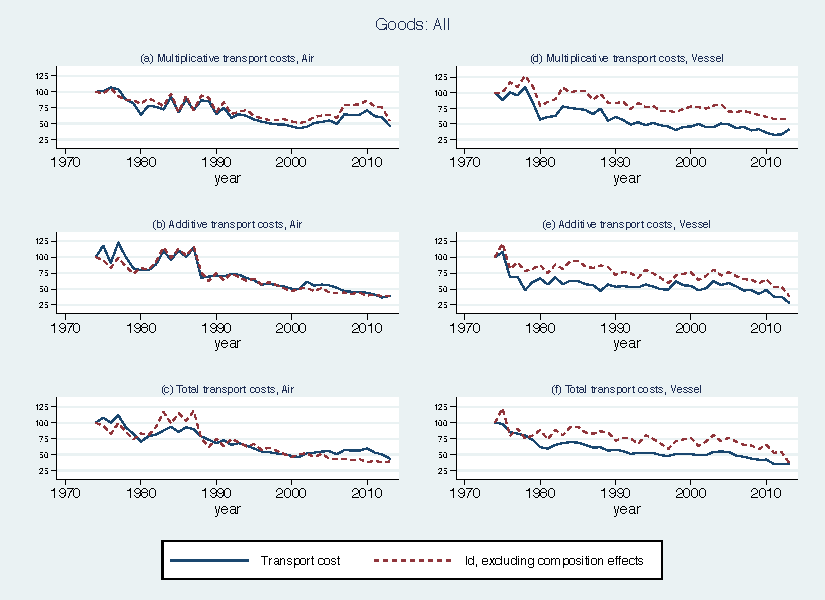
\includegraphics[height=4in]
{graph_composition_all.pdf}
\end{center}
\end{figure}


\textbf{Faire aussi une analyse plus fine par grande categorie: Manuf / Agriculture / Matieres premieres.}


Figure \ref{fig:totalTC_compeffects_excl} drives the following comments. Air transport costs were reduced by 50\% and vessel transport costs
by 60\%. (as already seen). However, in the case of vessel, a large part of that is a composition effect, probably because of the reduction in the share of bulky goods linked to the declining share of primary goods in total trade. The reverse happened for air transport : the goods shiped by air were increasingly more costly to transport. n line with \citet{hummels2007}, this confirms the importance of excluding these composition effects before assessing the time trends of transport costs.

(((At the agregate levelFirst, whatever the transport mode considered, transport costs have been roughly constant from 1974 to 1984. This stands in sharp contrast with Figures \ref{fig:mult_alone_withadd} and \ref{fig:decomp_TC_3d}, which rather conveyed the view that the fall in transport costs immediately started in 1974. Combining these results therefore indicates that the reduction of transport costs between 1974 and 1984 was due to changes in the composition of trade patterns (either in the country or the product dimension, or both) of the US, rather than a decrease in transport costs \textit{per se}. I

Second, after excluding the composition effects, we find that all types of transport costs have steadily decreased, to reach a reduction of 40\% over the period 1984-2011, in accordance with the literature. Further, if we only assume ad-valorem costs (Panel (a)), we can infer that the decrease is stronger for air transport than for air shipping over the period 1984-2005. This in accordance with the findings of \cite{hummels2007} and \cite{Behar_Venables}. Yet, going deeper in the decomposition between the additive and the ad-valorem components substantially modifies the picture, as it can be inferred from Panel (b). When the additive costs are taken into account, there is now not much difference in the reduction of transport costs between air transport and ocean shipping, and both display very similar time changes. The downward trend in transport costs indeed is roughly of the same order of magnitude throughout the years, for both transport modes. Taking into account the additive component therefore substantially modifies the analysis of the dynamics of transport costs over time. In Figure \ref{fig:TC_add_mult_compeffects_excl}, we investigate this result further, by reporting the changes in both the additive and ad-valorem components of transport costs, by transport mode.

\begin{figure}[htbp]
\caption{Decomposing transport costs over time,
composition effects excluded}
\label{fig:TC_add_mult_compeffects_excl}
\begin{center}
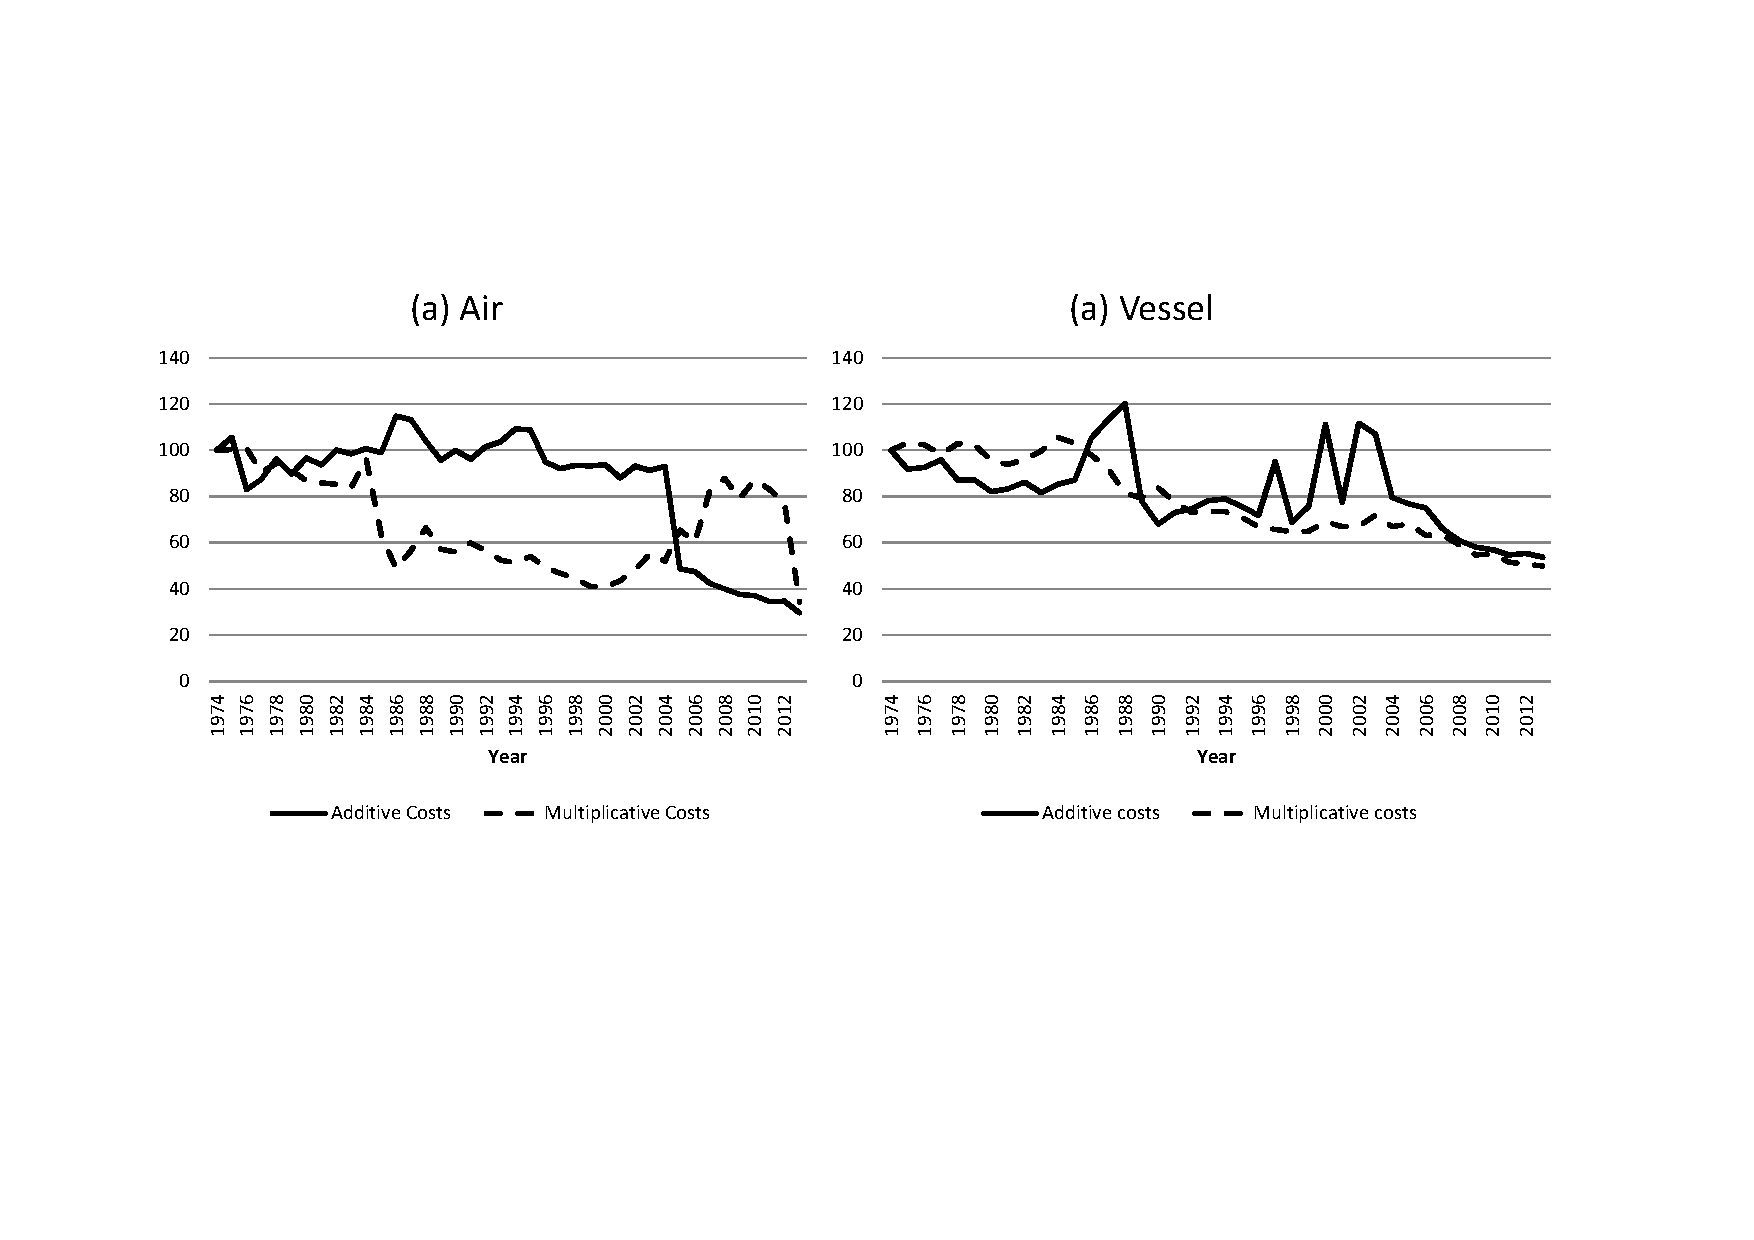
\includegraphics[width=14cm, height=7cm]{Fig3b_TCovertime_add_et_mult_3d.pdf}
%{\footnotesize {OECD data} }
\end{center}
\end{figure}

Again, the decomposition between both components of transport costs brings valuable insights. For ocean shipping, both additive and iceberg components exhibit a downward pattern since 1985. Air transport exhibit much more contrasted trends. While the ad-valorem component has been steadily declining over 1985-2000, the additive cost has been rather stable on the same period. Such a difference therefore most likely explains the difference of results between Panels (a) et (b) of Figure \ref{fig:totalTC_compeffects_excl}. Skipping the additive component leads to an important omission bias in the characterization of the time changes of transport costs. When correctly measured (ie, when the additive component is included), there is no noticeable difference in the downward trend of transport costs between ocean and air transport, in contradiction with the findings of \citet{hummels2007} and \cite{Behar_Venables}. Again, this finding points out to the importance of taking into account the additive component of international transport costs. \smallskip

Our analysis also brings valuable results to the findings of \citet{hummels2007}, as we extend his time coverage (end year 2004) by one decade (to stop in 2013). On this decade, our analysis reveals substantial changes in the time trend of transport costs in the air sector. As reported in Figure \ref{fig:totalTC_compeffects_excl}, Panel (b), transport costs have raised between 2005 and 2010, to substantially decline on the very recent years (2011-2013), by more than 20\%. As reported in Figure \ref{fig:TC_add_mult_compeffects_excl}, this can be attributed to the iceberg component (while the additive cost has conversely been drastically reduced since 2005). These results suggest that important changes in the structure of costs ate at work in the air transport in the very recent period, that should be investigated in further research.)))

\section{Robustness checks}

Robustness to the specification of the estimated equation. 


\paragraph{Robustness to the separability assumption}


Ie, estimate


$$\log(\frac{p_{ik}}{\widetilde{p}_{ik}} -1)= \log(\tau_{is} -1+ \frac{t_{is}}{\widetilde{p}_{ik}})+ \exp(\epsilon_{ik})$$

To do on 100 products ($s$), 50 countries (the most important?) 

\paragraph{what else?}

\section{Conclusion \label{sec:conclu}}

This paper empirically studies the magnitude of additive (or per-kg) costs in international transport costs, by exploiting the differences between the import and the export prices. Using SITC 3 and 4- digit cif-fas unit values taken from the US import database over 1974-2013, we estimate the two components of transport costs, by transport mode (air or ocean).  Our results may be summarized in three main findings. First, we provide a quantitative measure of both the additive and the iceberg transport cost. We thus find that additive costs amount to 2.8\% of the export price unit values for ocean shipping, and ad-valorem ones 3.2\%. These values are respectively equal to 1.8 and 2.5\% for air transport. Second, we show that taking additive costs into account improves the fit of the modelling of transport costs. All goodness-of-fit measures point out to this conclusion, which holds for both transport modes and all years considered. Third, we also use the time dimension of our data to characterize the evolution of transport costs. After correcting for composition effects, we find that all types of transport costs have been roughly constant from 1974 to 1984 and then steadily decreased by 40\% over the period 1984-2013. Yet, this steady decline hides shifts in the relative importance of additive and ad-valorem. While most of the early decline in air transport costs can be explained by the ad-valorem component, this component nearly doubled in the 2000s. Further, the inclusion of additive costs yields to the conclusion the decrease of overall trade costs are decreased in air transport and ocean shipping roughly the same path and the same magnitude of order. This last result stands in contrast with related studies (\citealp{hummels2007}, \citealp{Behar_Venables}). In all three aspects, our results point the importance of the additive component in accounting for international transport costs.

Our results could be extended in two main ways. On the empirical side, one may want to ge deeper in the ``structural'' determinants of trade costs, i.e. identify the respective roles of handling costs, insurance and freight at the root of the gap between export and import prices. On the theoretical side, our results can be used to explore the role of additive costs in shaping international trade flows (in an international trade theory perspective) and in affecting the international transmission of business cycles. This is left for further research.



\newpage
\bibliographystyle{essaien}
\bibliography{biblio}


\newpage


\appendix

\section{Data Appendix \label{app:data}}

\subsection{Fab-cif prices}

The Customs value is the value of imports as appraised by the U.S. Customs and Border Protection in accordance with the legal requirements of the Tariff Act of 1930, as amended. This value is generally defined as the price actually paid or payable for merchandise when sold for exportation to the United States, excluding U.S. import duties, freight, insurance, and other charges incurred in bringing the merchandise to the United States. The term ``price actually paid or payable'' means the total payment (whether direct or indirect, and exclusive of any costs, charges, or expenses incurred for transportation, insurance, and related services incident to the international shipment of the merchandise from the country of exportation to the place of importation in the United States) made, or to be made, for imported merchandise by the buyer to, or for the benefit, of the seller. In this respect, the ``custom value'' corresponds to the fas price (``free-alongside'' price) delivered by the seller.

The import charges represent the aggregate cost of all freight, insurance, and other charges (excluding U.S. import duties) incurred in bringing the merchandise from alongside the carrier at the port of exportation in the country of exportation and placing it alongside the carrier at the first port of entry in the United States. In the case of overland shipments originating in Canada or Mexico, such costs include freight, insurance, and all other charges, costs and expenses incurred in bringing the merchandise from the point of origin (where the merchandise begins its journey to the United States in Canada or Mexico to the first port of entry.

The cif (cost, insurance, and freight) value represents the landed value of the merchandise at the first port of arrival in the United States. It is computed by adding ``Import Charges'' to the ``Customs Value'' (see definitions above) and therefore excludes U.S. import duties.

\section{Some detailed results \label{app:more_results}}

In this section, we report the estimates for international transport costs, by transport mode on a yearly basis, when either additive costs are included in the estimation (Equation (\ref{eq:model_IetA})) or not (Equation (\ref{eq:model_nlI})). For sake of space saving, we only report the results for a sample of years. Tables \ref{tab:result_air_rob} and \ref{tab:result_ves_rob} display the results for the 4-digit product-level estimation (again, for selected years).


\begin{table}[htbp]
  \centering
  \caption{Air: Dynamics of Trade Costs over Time, 3 digits (selected years)}
\begin{center}
    \begin{tabular}{l|cccccc}
\hline\hline

Year & 1974  & 1980  & 1990  & 2000  & 2010  & 2013   \\ \hline
\multicolumn{7}{l}{\textbf{With only Iceberg Trade Costs}}     \\
Mean  & 1.069 & 1.054 & 1.050 & 1.036 & 1.042 & 1.034  \\
Median & 1.054 & 1.038 & 1.044 & 1.025 & 1.034 & 1.029  \\
Standard Error & 0.052 & 0.049 & 0.039 & 0.033 & 0.037 & 0.024 \\
\hline
\multicolumn{7}{l}{\textbf{With Additive \& Iceberg Trade Costs }}    \\
\multicolumn{1}{l}{\textit{Additive term }} &       &       &       &       &       &      \\
\multicolumn{1}{l}{Mean } & 0.026 & 0.020 & 0.018 & 0.013 & 0.011 & 0.010  \\
\multicolumn{1}{l}{Median} & 0.011 & 0.005 & 0.008 & 0.005 & 0.004 & 0.005  \\
\multicolumn{1}{l}{Standard Error} & 0.040 & 0.041 & 0.033 & 0.028 & 0.024 & 0.020  \\
\multicolumn{1}{l}{\textit{Iceberg term}} &       &       &       &       &       &        \\
\multicolumn{1}{l}{Mean } & 1.036 & 1.023 & 1.024 & 1.017 & 1.026 & 1.017  \\
\multicolumn{1}{l}{Median} & 1.027 & 1.016 & 1.016 & 1.012 & 1.022 & 1.017 \\
Standard Error & 0.032 & 0.025 & 0.021 & 0.016 & 0.023 & 0.012  \\ \hline
\# observations & 14955 & 16118 & 24958 & 35027 & 40279 & 39351  \\
\hline\hline
    \end{tabular}%
  \end{center}
  \label{tab:result_air_3d_detail}%
\tiny{Notes: Statistics are obtained weighting each observation by its value in transport (mode-dependent). Additive term expressed in fraction of fas price. }
\end{table}%


\begin{table}[htbp]
  \centering
  \caption{Vessel: Dynamics of Trade Costs over Time (3 digits), selected years}
\begin{center}
    \begin{tabular}{l|cccccc}
   \hline\hline
Year         & 1974  & 1980  & 1990  & 2000  & 2010  & 2013   \\
 \hline
   \textbf{With only Iceberg Trade Costs} &       &       &       &       &       &       \\
Mean  & 1.098 & 1.065 & 1.057 & 1.051 & 1.040 & 1.036  \\
Median & 1.096 & 1.055 & 1.046 & 1.049 & 1.036 & 1.033  \\
Standard Error & 0.053 & 0.040 & 0.032 & 0.028 & 0.020 & 0.018  \\
\textbf{With Additive \& Iceberg Trade Costs} &       &       &       &       &       &     \\
\hline
\textit{Additive term } &       &       &       &       &       &        \\
Mean  & 0.051 & 0.034 & 0.027 & 0.028 & 0.025 & 0.015  \\
Median & 0.029 & 0.023 & 0.017 & 0.022 & 0.019 & 0.008 \\
Standard Error & 0.085 & 0.046 & 0.040 & 0.043 & 0.025 & 0.020 \\
\textit{Iceberg term} &       &       &       &       &       &        \\
Mean  & 1.054 & 1.031 & 1.033 & 1.025 & 1.019 & 1.022 \\
Median & 1.049 & 1.024 & 1.028 & 1.021 & 1.018 & 1.018  \\
Standard Error & 0.041 & 0.023 & 0.022 & 0.021 & 0.018 & 0.018  \\
\hline
 \# obs & 19007 & 17356 & 28383 & 36090 & 37748 & 38473 \\ \hline
\hline\hline
    \end{tabular}%
  \end{center}
  \label{tab:result_ves_3d_detail}%
\tiny{Notes: Statistics are obtained weighting each observation by its value in transport (mode-dependent). Additive term expressed in fraction of fas price. }
\end{table}%



\begin{table}[htbp]
  \centering
  \caption{Air: Dynamics of Trade Costs over Time, 4-digit}
\begin{center}
    \begin{tabular}{l|cccccc}
   \hline\hline
Year & 1974  & 1981  & 1989  & 2001  & 2009  & 2013 \\
\multicolumn{7}{l}{\textbf{With only Iceberg Trade Costs} }  \\
Mean  & 1.066 & 1.058 & 1.052 & \multicolumn{1}{c}{1.033} & \multicolumn{1}{c}{1.037} & \multicolumn{1}{c}{1.032} \\
Median & 1.052 & 1.044 & 1.041 & \multicolumn{1}{c}{1.021} & \multicolumn{1}{c}{1.027} & \multicolumn{1}{c}{1.026}  \\
Standard Error & 0.056 & 0.054 & 0.046 & \multicolumn{1}{c}{0.040} & \multicolumn{1}{c}{0.036} & \multicolumn{1}{c}{0.025}  \\
\hline
\multicolumn{7}{l}{\textbf{With Additive \& Iceberg Trade Costs }}  \\ \hline
\textit{Iceberg term} &       &       &       &       &       &     \\
Mean  & 1.035 & 1.026 & 1.031 & \multicolumn{1}{c}{1.015} & \multicolumn{1}{c}{1.021} & \multicolumn{1}{c}{1.016}  \\
Median & 1.025 & 1.017 & 1.019 & \multicolumn{1}{c}{1.010} & \multicolumn{1}{c}{1.017} & \multicolumn{1}{c}{1.014}  \\
Standard Error & 0.036 & 0.028 & 0.030 & \multicolumn{1}{c}{0.021} & \multicolumn{1}{c}{0.024} & \multicolumn{1}{c}{0.015}  \\
\textit{Additive term} &       &       &       &       &       &     \\
Mean  & 0.026 & 0.021 & 0.017 & \multicolumn{1}{c}{0.012} & \multicolumn{1}{c}{0.012} & \multicolumn{1}{c}{0.010} \\
Median & 0.012 & 0.006 & 0.006 & \multicolumn{1}{c}{0.005} & \multicolumn{1}{c}{0.004} & \multicolumn{1}{c}{0.004}  \\
Standard Error & 0.039 & 0.042 & 0.033 & \multicolumn{1}{c}{0.027} & \multicolumn{1}{c}{0.029} & \multicolumn{1}{c}{0.019} \\ \hline
\# obs & 14944 & 16844 & 25307 & \multicolumn{1}{c}{35005} & \multicolumn{1}{c}{38475} & \multicolumn{1}{c}{39460}  \\
\hline\hline
    \end{tabular}%
  \end{center}
  \label{tab:result_air_rob}%
\tiny{Notes:Statistics are obtained weighting each observation by its value in transport (mode-dependent). Additive term expressed in fraction of fas price. }
\end{table}%


\begin{table}[htbp]
  \centering
\caption{Vessel: Dynamics of Trade Costs over Time, 4-digit}
\begin{center}
    \begin{tabular}{l|cccccc}
   \hline\hline
Year & 1974  & 1981  & 1989  & 2001  & 2009  & 2013 \\
\hline
\multicolumn{7}{l}{\textbf{With only Iceberg Trade Costs}} \\
Mean  & 1.098 & 1.061 & \multicolumn{1}{c}{1.058} & \multicolumn{1}{c}{1.051} & \multicolumn{1}{c}{1.042} & \multicolumn{1}{c}{1.036}  \\
Median & 1.094 & 1.051 & \multicolumn{1}{c}{1.048} & \multicolumn{1}{c}{1.045} & \multicolumn{1}{c}{1.038} & \multicolumn{1}{c}{1.031} \\
Standard Error & 0.060 & 0.038 & \multicolumn{1}{c}{0.036} & \multicolumn{1}{c}{0.030} & \multicolumn{1}{c}{0.023} & \multicolumn{1}{c}{0.020} \\
\hline
\multicolumn{7}{l}{\textbf{With Additive \& Iceberg Trade Costs } }\\ \hline
\textit{Iceberg term} &       &       &       &       &       &     \\
Mean  & 1.054 & 1.034 & \multicolumn{1}{c}{1.028} & \multicolumn{1}{c}{1.028} & \multicolumn{1}{c}{1.024} & \multicolumn{1}{c}{1.021}  \\
Median & 1.049 & 1.030 & \multicolumn{1}{c}{1.024} & \multicolumn{1}{c}{1.025} & \multicolumn{1}{c}{1.026} & \multicolumn{1}{c}{1.018} \\
Standard Error & 0.043 & 0.026 & \multicolumn{1}{c}{0.025} & \multicolumn{1}{c}{0.021} & \multicolumn{1}{c}{0.016} & \multicolumn{1}{c}{0.013}  \\
\textit{Iceberg term} &       &       &       &       &       &     \\
Mean  & 0.046 & 0.026 & \multicolumn{1}{c}{0.031} & \multicolumn{1}{c}{0.024} & \multicolumn{1}{c}{0.021} & \multicolumn{1}{c}{0.015}  \\
Median & 0.029 & 0.013 & \multicolumn{1}{c}{0.019} & \multicolumn{1}{c}{0.015} & \multicolumn{1}{c}{0.013} & \multicolumn{1}{c}{0.008} \\
Standard Error & 0.068 & 0.044 & \multicolumn{1}{c}{0.037} & \multicolumn{1}{c}{0.035} & \multicolumn{1}{c}{0.031} & \multicolumn{1}{c}{0.023} \\ \hline
\# obs & 19196 & 17916 & \multicolumn{1}{c}{29387} & \multicolumn{1}{c}{36677} & \multicolumn{1}{c}{37643} & \multicolumn{1}{c}{38820} \\
\hline\hline
    \end{tabular}%
  \end{center}
  \label{tab:result_ves_rob}%
\vspace{-10pt}\tiny{Notes: Statistics are obtained weighting each observation by its value in transport (mode-dependent). Additive term expressed in fraction of fas price. }
\end{table}%


\subsection{Goodness-of-fit: Detailed results \label{app:robust_4d}}

In this section, we report the goodness-of-fit exercise conducted by transport mode, for selected years at the 4-digit product classification level. The results are reported in Tables \ref{tab:good_fit_air_rob} (for Air) and \ref{tab:good_fit_ves_rob} (for Vessel), for a sample of some years.
\begin{table}[htbp]
  \centering
  \caption{Air: Measures of Goodness-of-fit, 4-digits}
\begin{center}
\label{tab:good_fit_air_rob}%
%\vspace{0.5cm}
\scalebox{0.97}{
\begin{tabular}{lcccccc}
\hline
\hline
      & \multicolumn{5}{c}{Year}                      &  \\
      & \multicolumn{1}{c}{1974} & \multicolumn{1}{c}{1981} & \multicolumn{1}{c}{1989} & \multicolumn{1}{c}{2001} & \multicolumn{1}{c}{2009} & \multicolumn{1}{c}{2013}  \\
\hline
\textbf{R2} & \multicolumn{1}{c}{} & \multicolumn{1}{c}{} & \multicolumn{1}{c}{} &       &       &      \\
Term I only & \multicolumn{1}{c}{0.48} & \multicolumn{1}{c}{0.49} & \multicolumn{1}{c}{0.50} & \multicolumn{1}{c}{0.50} & \multicolumn{1}{c}{0.45} & \multicolumn{1}{c}{0.35} \\
Terms A \& I & \multicolumn{1}{c}{0.63} & \multicolumn{1}{c}{0.66} & \multicolumn{1}{c}{0.65} & \multicolumn{1}{c}{0.66} & \multicolumn{1}{c}{0.54} & \multicolumn{1}{c}{0.45} \\
\textbf{SER} & \multicolumn{1}{c}{} & \multicolumn{1}{c}{} & \multicolumn{1}{c}{} &       & \multicolumn{1}{c}{} & \multicolumn{1}{c}{}  \\
Term I only & \multicolumn{1}{c}{} & \multicolumn{1}{c}{} & \multicolumn{1}{c}{} &       & \multicolumn{1}{c}{0.88} & \multicolumn{1}{c}{0.93}  \\
Terms A \& I & \multicolumn{1}{c}{} & \multicolumn{1}{c}{} & \multicolumn{1}{c}{} &       & \multicolumn{1}{c}{0.80} & \multicolumn{1}{c}{0.86}  \\
\textbf{Log-likelihood} & \multicolumn{1}{c}{} & \multicolumn{1}{c}{} & \multicolumn{1}{c}{} &       & \multicolumn{1}{c}{} & \multicolumn{1}{c}{} \\
Term I only & \multicolumn{1}{c}{-17505.55} & \multicolumn{1}{c}{-21813.46} & \multicolumn{1}{c}{-30960.56} & \multicolumn{1}{c}{-44067.62} & \multicolumn{1}{c}{-49375.57} & \multicolumn{1}{c}{-53197.87}  \\
Terms A\& I & \multicolumn{1}{c}{-14895.81} & \multicolumn{1}{c}{-18589.91} & \multicolumn{1}{c}{-26553.53} & \multicolumn{1}{c}{-37297.93} & \multicolumn{1}{c}{-45747.57} & \multicolumn{1}{c}{-49899.14}  \\
\textbf{AIC criteria} & \multicolumn{1}{c}{} & \multicolumn{1}{c}{} & \multicolumn{1}{c}{} &       & \multicolumn{1}{c}{}  \\
Term I only & \multicolumn{1}{c}{36243.10} & \multicolumn{1}{c}{44966.91} & \multicolumn{1}{c}{63417.12} & \multicolumn{1}{c}{89747.24} & \multicolumn{1}{c}{100317.13} & \multicolumn{1}{c}{107963.73} \\
Terms A \& I & \multicolumn{1}{c}{31873.63} & \multicolumn{1}{c}{39495.82} & \multicolumn{1}{c}{55777.05} & \multicolumn{1}{c}{77439.85} & \multicolumn{1}{c}{94059.14} & \multicolumn{1}{c}{102224.28}  \\
\textbf{Test LL} &       &       &       &       &       &       \\
2$\times$(ll(UR) -ll(R)) & \multicolumn{1}{c}{5219.47} & \multicolumn{1}{c}{6447.09} & \multicolumn{1}{c}{8814.06} & \multicolumn{1}{c}{13539.39} & \multicolumn{1}{c}{7255.99} & \multicolumn{1}{c}{6597.45}  \\
\# restrictions  & \multicolumn{1}{c}{640} & \multicolumn{1}{c}{698} & \multicolumn{1}{c}{778} & \multicolumn{1}{c}{833} & \multicolumn{1}{c}{824} & \multicolumn{1}{c}{818}  \\
p-value & \multicolumn{1}{c}{0.000} & \multicolumn{1}{c}{0.000} & \multicolumn{1}{c}{0.000} & \multicolumn{1}{c}{0.000} & \multicolumn{1}{c}{0.000} & \multicolumn{1}{c}{0.000} \\
\hline\hline
\end{tabular}}%
\end{center}
 \vspace{-10pt} \tiny{Notes: R$^{2}$ between the log of predicted ratio and the log of the observed ratio. The number \# of restrictions is equal to the number of parameters estimated, i.e., the number of partner countries plus the number of products.}
\end{table}%

\begin{table}[htbp]
  \centering
  \caption{Vessel: Measures of Goodness-of-fit, 4-digits}
\begin{center}
\label{tab:good_fit_ves_rob}%

\scalebox{0.97}{\begin{tabular}{l|cccccc}
\hline
\hline
      & \multicolumn{6}{c}{Year}                   \\
      & \multicolumn{1}{c}{1974} & \multicolumn{1}{c}{1981} & \multicolumn{1}{c}{1989} & \multicolumn{1}{c}{2001} & \multicolumn{1}{c}{2009} & \multicolumn{1}{c}{2013}  \\ \hline
\boldmath{}\textbf{R$^{2}$}\unboldmath{} &       &       &       &       &       &         \\
Term I only & 0.50  & 0.45  & \multicolumn{1}{c}{0.47} & \multicolumn{1}{c}{0.41} & \multicolumn{1}{c}{0.37} & \multicolumn{1}{c}{0.35} \\
Terms A \& I & 0.66  & 0.62  & \multicolumn{1}{c}{0.62} & \multicolumn{1}{c}{0.58} & \multicolumn{1}{c}{0.51} & \multicolumn{1}{c}{0.46} \\
\textbf{SER} &       &       & \multicolumn{1}{c}{} & \multicolumn{1}{c}{} & \multicolumn{1}{c}{} & \multicolumn{1}{c}{} \\
Term I only &       &       & \multicolumn{1}{c}{} & \multicolumn{1}{c}{} & \multicolumn{1}{c}{0.79} & \multicolumn{1}{c}{0.82} \\
Terms A \& I &       &       & \multicolumn{1}{c}{} & \multicolumn{1}{c}{} & \multicolumn{1}{c}{0.69} & \multicolumn{1}{c}{0.75} \\
\textbf{Log-likelihood} &       &       & \multicolumn{1}{c}{} & \multicolumn{1}{c}{} & \multicolumn{1}{c}{} & \multicolumn{1}{c}{} \\
Term I only & -16460.10 & -16951.61 & \multicolumn{1}{c}{-26771.44} & \multicolumn{1}{c}{-39008.34} & \multicolumn{1}{c}{-43888.90} & \multicolumn{1}{c}{-47161.62} \\
Terms A\& I & -12743.65 & -13546.92 & \multicolumn{1}{c}{-21752.77} & \multicolumn{1}{c}{-33280.96} & \multicolumn{1}{c}{-39078.86} & \multicolumn{1}{c}{-43399.22}  \\
\textbf{AIC criteria} &       &       & \multicolumn{1}{c}{} & \multicolumn{1}{c}{} & \multicolumn{1}{c}{} & \multicolumn{1}{c}{} \\
Term I only & 34464.19 & 35491.21 & \multicolumn{1}{c}{55272.87} & \multicolumn{1}{c}{79800.67} & \multicolumn{1}{c}{89459.80} & \multicolumn{1}{c}{95987.23}\\
Terms A \& I & 28271.29 & 29877.84 & \multicolumn{1}{c}{46595.55} & \multicolumn{1}{c}{69743.91} & \multicolumn{1}{c}{81155.73} & \multicolumn{1}{c}{89692.44} \\
\textbf{Test LL} &       &       & & &  & \\
2$\times$(ll(UR) -ll(R)) & 12385.80 & 11226.75 & \multicolumn{1}{c}{17354.65} & \multicolumn{1}{c}{20113.52} & \multicolumn{1}{c}{16608.16} & \multicolumn{1}{c}{12589.59} \\
\# restrictions  & 797   & 814   & \multicolumn{1}{c}{881} & \multicolumn{1}{c}{910} & \multicolumn{1}{c}{886} & \multicolumn{1}{c}{874} \\
p-value & 0.000 & 0.000 & \multicolumn{1}{c}{0.000} & \multicolumn{1}{c}{0.000} & \multicolumn{1}{c}{0.000} & \multicolumn{1}{c}{0.000} \\
\hline\hline
\end{tabular}}
\end{center}
  \vspace{-10pt}\tiny{Notes: R$^{2}$ between the log of predicted ratio and the log of the observed ratio. The number \# of restrictions is equal to the number of parameters estimated, i.e., the number of partner countries plus the number of products.}
\end{table}%

\section{More on eliminating the composition effects \label{app:comp-effects}}

In this section, we explain with more details the method employed to eliminate the country- and product- dimensions of the estimated transport cost. 

\paragraph{For the ad-valorem component} Consider first the multiplicative transport cost component. Rewriting Equation (\ref{eq:compeffects_mult}) by taking the exponential, we get:

\begin{equation*}
\widehat{\tau}_{ikt}=\exp\left(\delta + \sum_{i \neq \text{AFG}}\alpha_i.\mathbb{1}_i+\sum_{k\neq \text{011}}\beta_k.\mathbb{1}_k\right).\exp\left(\sum_{t \neq 1974}\gamma_t.\mathbb{1}_t\right) .\exp\left(\epsilon_{ikt}\right)
\end{equation*}

Based on this equation, we deduce after estimation that: 
\begin{eqnarray*}
\text{For the year 1974}&& \widehat{\tau}_{is74} = \exp(\delta +\alpha_i+\beta_s), \\
\text{For any year}~t> 1974&& \widehat{\tau}_{ist} = \exp(\delta +\alpha_i+\beta_s)\times \exp(\gamma_t)
\end{eqnarray*} 

From this, we obtain the foolowing recursive link: $\widehat{\tau}_{ist} = \widehat{\tau}_{is74}\exp(\gamma_t)$. Given that $\tau >1$, we can rewrite things to get the percentage change between year 1974 and any year $t>1974$:
$$\Gamma_{ist} = 100.\frac{\widehat{\tau}_{ist}-1}{\widehat{\tau}_{is74}-1} = 100.\frac{\widehat{\tau}_{is74}\exp(\gamma_t)-1}{\widehat{\tau}_{is74}-1}$$

As such, the index of transport costs in year $t$ (relative to the reference year 1974) $\Gamma_{ist} $  only depends on the cost observed in 1974 and the time trade. At this stage though, it remains specific to a product-origin country pair. Next step is to build the index $\Gamma_t$ such that:
\begin{equation*}
 \Gamma_t= 100.\frac {\bar{\tau}_{1974}.\exp(\gamma_t)-1} {\bar{\tau}_{1974}-1}
\end{equation*}
\noindent with $\bar{\tau}_{1974} = \exp(\delta + \sum_i \alpha_i + \sum_k \beta_k$) the mean (ad-valorem) transport cost in 1974. 

\paragraph{For the additive component} After estimating Equation (\ref{eq:compeffects_add}), we can re-build the additive component according to:
\begin{eqnarray*}
\text{For the year 1974}&&\widehat{t}_{is74}=  \delta + \alpha_i+ \beta_s, \\
\text{For any year}~t> 1974&&\widehat{t}_{ist}=\left(\delta + \alpha_i+ \beta_s\right).\exp(\gamma_t)
\end{eqnarray*}

From this, we deduce the recursive link: $\widehat{t}_{ist} = \widehat{t}_{is74} \times \exp(\gamma_t)$. Given the contraint $t>0$, we then obtain the percentage change from 1974 from:

\begin{equation*}
\Gamma^{add}_{ist} = 100\frac{\widehat{t}_{ist}}{\widehat{t}_{ik74}} = 100\exp(\gamma_t)
\end{equation*}

Noticing that it is independent of the product-origin country pair, we can thus rewrite the time-trend series for the additive transport cost component as:
$$\Gamma^{add}_t  = 100\exp(\gamma_t) $$

\end{document}

